%\pdfoutput=1
\documentclass[runningheads,draft]{llncs}
\usepackage{amsmath,amssymb,amsfonts}
%\usepackage{stmaryrd}       % Semantic brackets \llbracket and \rrbracket
%\usepackage{mathpartir}     % inference rules
\usepackage[scaled=0.8]{helvet}    % Less huge \textsf{functionName}
\usepackage{enumitem}       % compacts lists and stuff
\usepackage[subtle]{savetrees}
\usepackage{soul}           % \hl for highlighting text; \st for strike-through

\usepackage{graphicx}
\usepackage{xcolor}
\usepackage{tikz,tikzpeople}
\usetikzlibrary{trees,snakes,arrows}
\usepackage{environ}  % For tikz fig spanning two columns
\usetikzlibrary{positioning}
% Used for displaying a sample figure. If possible, figure files should
% be included in EPS format.
%
% If you use the hyperref package, please uncomment the following line
% to display URLs in blue roman font according to Springer's eBook style:
\usepackage{hyperref}
%\renewcommand\UrlFont{\color{blue}\rmfamily}
% not the way to do it for arXiv though...
\usepackage{url}
\hypersetup{
    final, % Uncomment to remove all links (useful for printing in black and white)
    colorlinks=true, breaklinks=true, bookmarks=false,bookmarksnumbered,
    urlcolor=blue, linkcolor=black, citecolor=green, % Link colors
%   pdftitle={title of paper}, % PDF title
%   pdfauthor={auth1, auth2}, % PDF Author
%   pdfsubject={}, % PDF Subject
    pdfkeywords={}, % PDF Keywords
    pdfcreator={PdfLaTeX}, % PDF Creator
%   pdfproducer={Pandoc, XeLaTeX with hyperref} % PDF producer
  }
\usepackage[final]{listings}

\definecolor{codegreen}{rgb}{0,0.6,0}
\definecolor{codegray}{rgb}{0.5,0.5,0.5}
\definecolor{codepurple}{rgb}{0.58,0,0.82}
\definecolor{backcolour}{rgb}{0.95,0.95,0.92}

\lstdefinestyle{mystyle}{
    backgroundcolor=\color{backcolour},   
    commentstyle=\color{codegreen},
    identifierstyle=\color{black},
    keywordstyle=\color{magenta},
    numberstyle=\scriptsize\color{codegray},
    stringstyle=\color{codepurple},
    basicstyle=\ttfamily\scriptsize\color{codegray},
    breakatwhitespace=false,
    breaklines=true,
    captionpos=b,
    keepspaces=true,
    numbers=left,
    numbersep=5pt,
    showspaces=false,
    showstringspaces=false,
    showtabs=false,
    tabsize=2,
%    literate={--[}{$-\hspace{-3pt}[$}{3}{]->}{$]\hspace{-3pt}\rightarrow$}{3},
    keywords={let,in,rule,restriction,axiom,lemma,all-traces,exists-trace,Ex,All,Fr,In,Out}
}

\lstset{style=mystyle}


\def\BibTeX{{\rm B\kern-.05em{\sc i\kern-.025em b}\kern-.08em
    T\kern-.1667em\lower.7ex\hbox{E}\kern-.125emX}}

%\usepackage{algorithm}
%\usepackage{algpseudocode}         % https://en.wikibooks.org/wiki/LaTeX/Algorithms#Typesetting_using_the_algorithmic_package

\usepackage{draftwatermark}
\SetWatermarkText{\textbf{DRAFT}}
\SetWatermarkScale{2}
\SetWatermarkColor[gray]{.92}


\usepackage[numbers, sort]{natbib}
\usepackage[T1]{fontenc} % E.g., for small caps in section headings
\usepackage{xspace}
\usepackage[lambda,advantage,operators,adversary,landau,probability,notions,logic,
ff,mm,primitives,events,complexity,asymptotics,sets,keys]{cryptocode}

% http://tug.ctan.org/tex-archkeIVe/macros/latex/contrib/todonotes/todonotes.pdf
\usepackage{todonotes}
\newcommand{\knote}[1]{\todo[inline,
                             color=orange,
                             size=\footnotesize
                         ]{\textsf{\textbf{Karl:} #1}}}
%\newcommand{\knote}[1]{}

% -- Fonts and styles for names
\newcommand{\mItemStyle}[1]{\ensuremath{#1}}
\newcommand{\mSetStyle}[1]{\ensuremath{\mathrm{\mathbf{#1}}}}
\newcommand{\mFunStyle}[1]{\text{\textup{\textsf{#1}}}}
\newcommand{\mConstStyle}[1]{\text{\textup{\textsf{#1}}}}
\newcommand{\mVarStyle}[1]{\mathit{#1}}
\newcommand{\mFactStyle}[1]{\text{\textsf{#1}}}
\newcommand{\mRuleStyle}[1]{\ensuremath{\mathbf{#1}}}
\newcommand{\mDomainStyle}[1]{\ensuremath{\mathcal{#1}}}



% Solution for letting a tikz figure to span two columns by Ulrike Fischer
% https://tex.stackexchange.com/questions/6388/how-to-scale-a-tikzpicture-to-textwidth
\makeatletter
\newsavebox{\measure@tikzpicture}
\NewEnviron{scaletikzpicturetowidth}[1]{%
  \def\tikz@width{#1}%
  \def\tikzscale{1}\begin{lrbox}{\measure@tikzpicture}%
  \BODY
  \end{lrbox}%
  \pgfmathparse{#1/\wd\measure@tikzpicture}%
  \edef\tikzscale{\pgfmathresult}%
  \BODY
}
\makeatother
%
\begin{document}
\title{EDHOC - Tamarin modeling paper}
\author{First Author\inst{1}\orcidID{0000-1111-2222-3333} \and
Second Author\inst{2,3}\orcidID{1111-2222-3333-4444} \and
Third Author\inst{3}\orcidID{2222--3333-4444-5555}
{\color{red} DRAFT: \today}
}
%
\authorrunning{F. Author et al.}
% First names are abbreviated in the running head.
% If there are more than two authors, 'et al.' is used.
%
\institute{
    KTH Royal Institute of Technology, SE-100 44, Stockholm, Sweden \and
    Ericsson Security Research, SE-164 83, Stockholm, Sweden,
    \email{karl.norrman@ericsson.com} \and
    ITU Copenhagen $\ldots$ \and
    Ericsson Intell. Autonomous sys$\ldots$
}
%
\maketitle
%

\begin{abstract}
\hl{250 words}
IETF is standardizing a key establishment protocol, named \mEdhoc, for
constrained IoT devices.
%
In contrast to more powerful IoT devices, such as video cameras and cars,
which receive most attention from media, constrained devices often have severe
restrictions on energy consumption.
%
Additionally, they often use specialized wireless communication links with tough
constraints on message sizes, which may vary from message to message.
%
\mEdhoc{} was first formally analyzed by
Bruni~et.~al.~\cite{DBLP:conf/secsr/BruniJPS18}.
%
Since then, IETF has significantly extended the protocol, which is now a
framework with a number of cryptographic cores, called methods, where the
initial version of \mEdhoc{} contained only two out of five possibilities.
%
In this paper we formally analyze all methods of \mEdhoc{} in a symbolic model,
using the \mTamarin{} verification tool.
%
We show that the different methods provide sensible, but also rather
heterogeneous security properties, and discuss consequences of this.
%
\end{abstract}
%
{\color{red}
    Time plan (we keep weekly Thursday meetings for sync):
\begin{itemize}
    \item \textbf{Target conference:} Security Standardization Research (SSR),
                               \hl{Submit DL: 24/8},
                               Notification: 1/10,
                               Camera ready: 12/10,
                               20 pages including bib, LCNS template
    \item \textbf{18/6} Outline and work division proposed by Karl; Karl and
        Vaishnavi start writing our parts
    \item \textbf{25/6} Alessandro can start writing his parts
    \item \textbf{\hl{9/7}} \mArxiv version ready for upload (minus formatting issues)
    \item \textbf{13/7} \mArxiv formatted version sent out for review (at least to
        Mads Dam, IETF team and internal Eri review).
    \item \textbf{17/7} Possible comments from review fixed, and upload to
        \mArxiv. This DL is needed. Otherwise people at the IETF meeting will
        not be able to comment from the IETF meeting.
    \item \textbf{---} Vacation(...)
    \item \textbf{20/8} Reformatted to SSR 2020 LNCS; Possibly added properties
        to model and paper if something useful came up during vacation
    \item \textbf{24/8} SSR submission deadline
\end{itemize}
}

%\scalebox{.7}{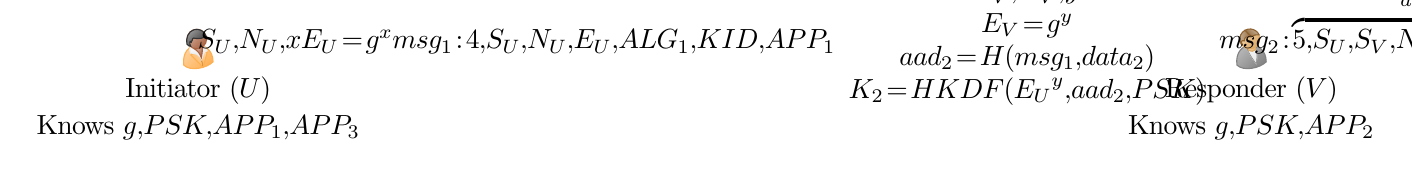
\begin{tikzpicture}[people/.style={minimum width=1em}]
    \node[people, alice] (ini) {Initiator ($U$)};
    \node[below of=ini] () {Knows $g, PSK, APP_1, APP_3$};
    \node[people, bob, right=13cm of ini] (res) {Responder ($V$)};
    \node[below of=res] () {Knows $g, PSK, APP_2$};
    
    \action{3em}{ini}{Generates $S_U,\ N_U,\ x$\\$E_U = g^{x}$};
    
    \msg{7em}{ini}{res}{$msg_1: 4,\ S_U,\ N_U,\ E_U,\ ALG_1,\ KID,\ APP_1$};
    \action{8em}{res}{$
      \begin{array}{c}
        \text{Generates }S_V,\ N_V,\ y\\
        E_V = g^{y}\\
        aad_2 = H(msg_1, data_2)\\
        K_2 = HKDF({E_U}^{y},\ aad_2,\ PSK)
      \end{array}$};
    \msg{16em}{res}{ini}{$msg_2: \overbrace{5,\ S_U,\ S_V,\ N_V,\ E_V,\ ALG_2}^{data_2},\ enc_{K_2}^{aad_2}(APP_2)$};
    \action{17em}{ini}{$
      \begin{array}{c}
        K_2 = HKDF({E_V}^{x},\ aad_2,\ PSK)\\
        aad_3 = H(H(msg_1, msg_2), data_3)\\
        K_3 = HKDF({E_V}^{x},\ aad_3,\ PSK)
      \end{array}$};
    
    \msg{24em}{ini}{res}{$msg_3: \overbrace{6,\ S_V}^{data_3}, aead_{K_3}^{aad_3}(APP_3)$};
    \action{25em}{res}{$K_3 = HKDF({E_U}^{y},\ aad_3,\ PSK)$};
    \end{tikzpicture}}

%-------------------------------------------------------------------------- sec
{\color{blue}
\section*{Outline}
This section is only for the outline and will be removed in the final
    paper. Don't worry about the language or style. Only the content matters.
\vspace{10pt}
\knote{Please do use and define macros in the file \texttt{macros.tex}!}
\knote{Notes like this one are defined for the macros
    \texttt{\textbackslash knote},
    \texttt{\textbackslash vnote} and
    \texttt{\textbackslash anote}}

\begin{itemize}
    \item \textbf{Section: Situation and setting (\hl{Karl})}
        \begin{itemize}
            \item OK: Elaborate on the story line above
            \item OK: Explain the exploratory and iterative nature of industrial
                  standards and why this has resulted in the new \mStat methods.
            \item OK: Contrast with \mTls. Motivate why \mEdhoc{} is needed in
                addition to \mTls. Little analysis of \mEdhoc{} so far.
                Motivate that most security analysis and media attention is on
                larger IoT devices. Give examples and cite use cases whit
                constrained devices. Paint the (true) picture that this will
                become a serious security risk in the future if not a secure
                \mEdhoc{} is created.
            \item OK: Subsection: Contributions: model, verified properties,
                guidance on how various methods can be used (for std and
                implementations)
            \item OK: Subsection: Related work: \mOptls, \mNoise,
                Bruni~\cite{DBLP:conf/secsr/BruniJPS18}, Cremers' et. al. \mTls
                analysis with \mTamarin.
        \end{itemize}
    \item \textbf{Section: \mEdhoc{} description (\hl{Vaishnavi})}
        \begin{itemize}
            \item Describe evolved protocol from last \mEdhoc{} verification,
            \item Describe the overarching goal of \mEdhoc{} of security context
                establishment for \mEdhoc.
            \item Describe that \mEdhoc{} is a framework based on three different
                crypto-cores (\mPsk-based DH, \mSigma and \mOptls/\mNoise).
                Some inital thoughts on \mNoise here~\ref{sec:mail-notes-noise}.
                Describe how one party may use a \mSigma-like authentication
                whereas the other party may use \mOptls. The session key is
                the combination of the corresponding key material.
                Describe that this essentially makes
                \mEdhoc{} a framework where it is possible to run one out of 5
                different protocols.
            \item Describe \mSigSig method and relate it to original \mEdhoc{} and
                \mSigma. This can be brief. Identify and focus on potential
                differences.
            \item Describe \mPskPsk method.
            \item Main focus of this section. Describe \mStat based methods, which
                  have very different properties compared to original \mEdhoc,
                  which only had the single \mSigma method.
                  Draw a figure (use tikz for easiest handling), showing how the
                  protocols look like (\mStatStat, \mStatSig, \mSigStat are
                  sufficient, the \mPsk and \mSigSig methods are simpler/old and
                  less interesting).
                  Explain the difference in signatures: "Normal" vs. challenge
                  response signatures of \mStat-based method.
                  Explain how \mStatStat is basically running two interleaved
                  \mOptls protocols runs. Compare how \mStat based methods relate
                  to \mOptls and to relevant instance from \mNoise framework.
                  Make mapping as precise as possible, down to key derivation
                  inputs. If the mapping of protocol elements and inputs to
                  key derivations and other processing is sufficiently close,
                  then point to security proof for Noise and cite it. Otherwise
                  point out the differences.
             \item Describe additional components of \mEdhoc{} we've modeled,
                  e.g., \mCi and \mCr etc.
                  Explain relevance of \mCi and \mCr to \mOscore.
             \item Describe algorithm negotiation.
             \item Describe negotiation of method.
             \item Describe transmission of aux data and expected security
                 properties.
        \end{itemize}
    \item \textbf{Section: \mEdhoc{} security model and formalization (\hl{Alessandro})}
        \begin{itemize}
            \item Subsection: threat model. We assume secure binding between
                credentials and the identity. We assume adversary cannot
                register another key for a name for an uncorrupted party. We
                assume adversary has Dolev-Yao style access to communication
                between agents. We assume adversary can compromise session keys,
                but is then not allowed to "test" that session key (in
                computational terminology). We assume adversary can compromise
                parties, but is not allowed to "test" them or their partners if
                he has done so. Two peers are partnered if they agree on: Their
                identities, and the session key material (except \mGiy in the
                relevant cases of \mStat). That is the session identifier and it
                is unique per run, which the injective agreement lemmas show.
                Define what is the key material for each method
                (see the \mTamarin model).
            \item Subsection: Short description of \mTamarin. It is known by
                now, but a short overview does not hurt.
            \item Subsection: Explain details of model, which properties we have
                modeled, how, which trade-offs were made and why.
                Explain how we modeled inj-agree (a sentence or two). Explain
                why it fails when $I$ uses \mStat-method and the implicit auth
                lemma we showed instead
                (cite~\cite{DBLP:journals/iacr/GuilhemFW19} here where I got the
                basic idea. It is then extended with the reveal queries in our
                model; obviously: if you know about other sources for this
                please cite them too). Include code/lemmas as you see fit.
            \item Subsection: Clear bullet-list of what we have shown, including
                some statics of running time code size perhaps.
                Scan draft-selander and check what props are claimed there; see
                what we have covered and what we haven't.
                Already shown:
                \begin{itemize}
                    \item Mutual injective agreement on session key, method and identities for
                        $R \rightarrow I$ and $I \rightarrow R$ for all methods
                        except when $I$ uses STAT. When $I$ uses STAT, $R \rightarrow I$ holds,
                        but not $I \rightarrow R$.
                    \item Injective implicit agreement on session key.
                        Only really needed for $I \rightarrow R$, because in all other cases we have
                        the stronger injective agreement property. But show it now for all
                        methods to having a common (and reasonable) level of security that
                        holds no matter which method user chooses.
                    \item PFS on session key for all methods.
                    \item Key secrecy (follows from PFS).
                    \item Session key independence (follows from how we modeled PFS).
                    \item Entity authentication - we show this in the same lemmas as we show
                          inj-agree on session key.  We don't have this property when $I$ uses
                          STAT method because $I$ then gets no confirmation of
                          Pre-specified peer model.
                    \item Key confirmation (except for when $I$ uses \mStat
                        method, then $I$ gets no key confirmation on \mGiy)
                \end{itemize}
            \item See~\ref{sec:mail-notes-encr} for how encryption is modeled.
            \item Caveat: we have not modeled running all methods in parallel,
                so we don't know if an adversary can somehow trick $I$ into
                running one method and $R$ another, and by that causing some
                attack.
        \end{itemize}
    \item \textbf{Section: Discussion (\hl{Karl})}
        \begin{itemize}
            \item{\textbf{Design practices}}
                \begin{itemize}
                \item OK. Discuss that the security properties varies between methods
                and that this may confuse implementers and user of libraries.
                \item OK. Discuss practice of listing claimed properties (likely copied
                from some academic paper) without justification in IETF drafts.
                \end{itemize}
            \item{\textbf{\mGiy and technical protocol issues}}
                \begin{itemize}
                \item Discuss unclearity regarding security model (trusted execution
                environment or not?). \mOptls has clear separation and therefore
                use both $g^{xy}$ and $g^{iy}$ etc. \mEdhoc{} is not as cleanly
                designed and according to IETF guys they don't care about
                trusted execution environments (see mail in txt-file).
                Would \mEdhoc{} be OK with skipping $g^{iy}$ from the session key
                material and only use $g^{xy}$ in that model? Probably yes, and
                then we can get inj-agree on the session key material, but then
                extending \mEdhoc{} implementations with a trusted execution
                environment for LTK operations is useless.
                \item OK: Discuss algorithm negotiation.
                \item OK: Discuss what should be used as session key and what the
                consequences of the choices are,
                see~\ref{sec:mail-notes-secrecy-sessions} and
                \ref{sec:mail-notes-session-key-mtrl}.
                \item OK: Discuss session key authentication and the problem of \mGiy,
                see~\ref{sec:mail-notes-session-key-auth}
                and~\ref{sec:mail-notes-session-key-imp-auth}
                \item OK: Discuss non-repudiation that was not included until we pointed
                it out.
                \item OK: Discuss the overlayed \mOptls construction and how an
                additional \mOscore message $R \rightarrow I$ would give key
                confirmation and hence explicit inj-agree also for $I$.
                \item Discuss Transcipt hashes that lag behind one message and that
                it is supposed to "cover as much as possible", but sometimes
                does not (check tamarin model also for inconsistencies between
                methods). Unclear design except "as much as possible".
                \end{itemize}
            \item{\textbf{Protocol user/implementor issues}}
                \begin{itemize}
                \item OK: Discuss Identities and use-cases with the neighbours printer
                (now included in draft, but only after we mentioned it),
                See~\ref{sec:mail-notes-identity}.
                \end{itemize}
        \end{itemize}
\end{itemize}
}

%-------------------------------------------------------------------------- sec
\section{Introduction}
\label{sec:introduction}
%-------------------------------------------------------------------------- sub
\subsection{Background and motivation}
\label{sec:motivation}
IoT security threats involving cars, web-cameras and other resourceful devices
receive most attention from media and academia.
%
These devices are computationally strong with no severe bandwidth or energy
consumption restrictions.
%
Securing the communication between such devices can readily be done using
\mDandTls.
%
Constrained devices, on the other hand, where such restrictions are common,
have received much less attention.
%
These devices may be simple sensors with the only task of relaying
measurements of their physical environment to a server every hour, and doing so
autonomously for a decade without maintenance.
%
Constrained devices therefore often have limitations on energy consumption.
%
To keep energy consumption down, highly specialized radio links with small
and heterogeneous frame-sizes are sometimes used.
%
In some cases, \mDandTls{} messages are too large to fit into the radio frames.
%
This is one of the reasons IETF standardized the \mOscore{} protocol to secure
communications between constrained devices, as a complement for when
\mDandTls{} is too heavy weight~\cite{rfc8613}.
%

The \mOscore{} protocol requires a pre-established security context.
%
The IETF Lightweight Authenticated Key Exchange (LAKE) working group
currently develops requirements and a key exchange protocol capable of
establishing \mOscore{} security contexts.
%
The key establishment protocol is named \mEdhoc~\cite{selander-lake-edhoc-01}.
%
Naturally, \mEdhoc{} must work under the same constrained requirements as
\mOscore{} itself.
%

While neither the requirements nor the use-cases for \mEdhoc{} are firmly set,
the overarching design goal of \mEdhoc{} is to establish an \mOscore{} security
context with decent security while keeping the messages small.
%
The LAKE working group is currently discussing whether a compressed version of
\mTls, named \mCtls~\cite{ietf-tls-ctls-00}, would solve the same use-cases as
\mOscore{} and \mEdhoc{} combined.
%

The \mEdhoc{} protocol has evolved significantly over time to cater for smaller
messages and more use-cases.
%
The first incarnation of \mEdhoc{} appeared in March 2016.
%
It contained two different cryptographic cores, one based on a
pre-shared key Diffie-Hellman and a second following a draft of the
then emerging \mbox{\mTls{} v1.3} standard~\cite{ietf-tls-tls13-11}, using
challenge-response signatures.
%
The latter was then replaced by \mSigma, and this version, from May 2018, was
formally analyzed by Bruni~et.~al.~\cite{DBLP:conf/secsr/BruniJPS18}.
%
The protocol has now further evolved and variants using challenge-response
signatures have now been added again.
%
On top of this, mixed variants where one party uses a challenge-response
signature and the other a regular signature have also been added.
%
Consequently, there are now five cryptographic cores in total, and it is prudent
to formally analyze them all to ensure a higher level of security assurance for
\mEdhoc.
%
This is especially important, since the \mSpec{} itself lacks description of the
intended security model and overall security goals.
%
Filling this gap and deriving circumstances under which \mEdhoc{} can be
securely used to achieve certain goals is an important part of this paper.
%

%-------------------------------------------------------------------------- sub
\subsection{Contributions}
\label{sec:contributions}
Our main contributions are the following.
\begin{itemize}
    \item We provide formalization of \mEdhoc's all five cryptographic cores
        using\linebreak \mTamarin~\cite{DBLP:conf/cav/MeierSCB13}.
    \item We give an explicit security model for the protocol and have verified
        essential security properties, such as session key and entity
        authentication, as well as Perfect Forward Secrecy (PFS), within that
        model.
    \item We provide consequence analysis of the verified properties to
        establish which types of use-cases \mEdhoc{} may be suitable for and
        to give recommendations for the future standards development.
    \item Our discussions with IETF LAKE working group members have already
        lead to improvements and clarifications of the standard \mSpec{} based
        on observations we made during the construction of our formal model.
\end{itemize}

%-------------------------------------------------------------------------- sub
\subsection{Related work}
\label{sec:relatedWork}
The work closest to ours is Bruni~et. al.~\cite{DBLP:conf/secsr/BruniJPS18},
which used \mProverif~\cite{DBLP:conf/csfw/Blanchet01} to analyze an earlier,
two cryptographic core, version of \mEdhoc.
%
We consider our work to be a sort of follow-up to that, doing a similar kind of
analysis of the most recent, and more elaborate, version of \mEdhoc{} using five
cores.
%
We also verify slightly different properties.
%
For instance, we include session key independence in our properties.
%
The \mTamarin{} tool has been used to verify many other protocols, perhaps closest
to our work is Cremers~et.~al's analysis of
\mTls~\cite{DBLP:conf/ccs/CremersHHSM17}.
%
Some of the cryptographic cores themselves have been analyzed in the
computational model, e.g., \mSigma{} by Canetti and
Krawczyk~\cite{DBLP:conf/crypto/CanettiK02} and \mOptls{} by Krawczyk and
Wee~\cite{DBLP:conf/eurosp/KrawczykW16}.
%
\knote{Add work on \mNoise{} here when Vaishnavi has added her section.}

%-------------------------------------------------------------------------- sub
\subsection{Structure}
\label{sec:structure}
\knote{Only include this if we have space to spare.}

%-------------------------------------------------------------------------- sec
\section{The \mEdhoc{} protocol}
\label{sec:edhoc}
\hl{Vaishnavi}
% !TEX root =  main.tex

%Description of \m\mEdhoc and main changes from last verified version

\vnote{Note for discussion with others: I find the macros for the protocol, method, and tool names distracting while reading through (the font changes too much, too often). The macro for EDHOC actually inserts a line break if you start a sentence with it, because of the \texttt{hbox} (I'm not sure why the hbox exists for what is a macro to be inserted in running text). I do need to start sentence with EDHOC many times though, so this is irritating. It is also the case that ProVerif needs to be written like so, and not capitalized entirely, so at least one of them is plain wrong! For now I've left in the macros, but I'd prefer that we fixed them to be regular capitalized text or, in the case of ProVerif, in camelcase as they should be.}

\vnote{Macros don't work right in section headers!}

\subsection{Overview}
Constrained IoT systems often deal with a lot of valuable personal and business information that ought to be kept secure. Such systems need to be assured of end-to-end protection with source authentication and perfect forward secrecy. It is often desirable to protect such devices at the application layer -- for example, in cases where transport layer security is not sufficient [\mcneed], or where multiple underlying protocols need to be accounted for. One method for providing application layer security is provided by CBOR Object Signing and Encryption (\mCose) [RFC8152: \mcfix].  

In order to derive shared key material with which to proceed, communicating parties can run an Elliptic Curve Diffie-Hellman key exchange protocol with ephemeral keys. Ephemeral Diffie-Hellman Over \mCose (\mEdhoc) is a lightweight key exchange protocol for such situations, and is expected to provide perfect forward secrecy and identity protection. \mEdhoc supports authentication using pre-shared keys (PSK), raw public keys (RPK), and public key certificates. After successful completion of the \mEdhoc protocol, application keys and other application specific data can be derived using the \mEdhoc-Exporter interface. 

A main use case for \mEdhoc is to establish a security context for Object Security for Constrained RESTful Environments (\mOscore) [RFC8613: \mcfix]. \mOscore is a protocol which uses \mCose for application-layer protection on top of the transport-layer Constrained Application Protocol (CoAP). \mEdhoc uses \mCose for cryptography, CBOR for encoding, and CoAP for transport. By reusing existing libraries, the additional code footprint can be kept very low.

\mEdhoc is designed to work in highly constrained scenarios. This makes it especially suitable for network technologies which have low throughput, low power consumption, and small frame sizes. Examples include Cellular IoT, 6TiSCH, and LoRaWAN [\mcneed].

The \mEdhoc protocol can establish Diffie-Hellman key exchange in one of three different ways -- using digital signatures, static Diffie-Hellman (DH) keys, or pre-shared symmetric keys. We describe each of these methods in detail below. The communicating parties must agree on the method and cipher suite used for encryption as part of the first message. The parties exchange ephemeral public keys, compute the shared secret, and derive symmetric application keys from this secret.

The \mSigma (SIGn-and-MAc) family of protocols [\mcneed] has many variants. The \mSig-based methods of \mEdhoc are built on \mSigmaI, a variant of the \mSigma protocol which provides identity protection for the initiator, and  implements the \mSigmaI variant as Mac-then-Sign. The method involving static DH keys proceeds along the lines of \mOptls, with the agent creating a MAC and encrypting it using an algorithm for authenticated encryption with associated data (\mAead) [\mcneed]. 

\mEdhoc allows the initiator and responder to run different methods, combining \mSig and \mStat -- for example, the initiator might run a \mSig-based method, while the responder is running a \mStat-based method. This set of methods is not covered in previous versions of \mEdhoc, which only had a single \mSigma asymmetric key method (corresponding to the \mSigSig method shown in Section~\ref{sec:methods}). This allows one party to use a \mSigma style of authentication using signatures, while the other can use static DH keys. In Figure~\ref{fig:edhocasym}, a template for all the asymmetric key methods of EDHOC is shown. 

\begin{figure}[!h]\label{fig:edhocasym}
\centering
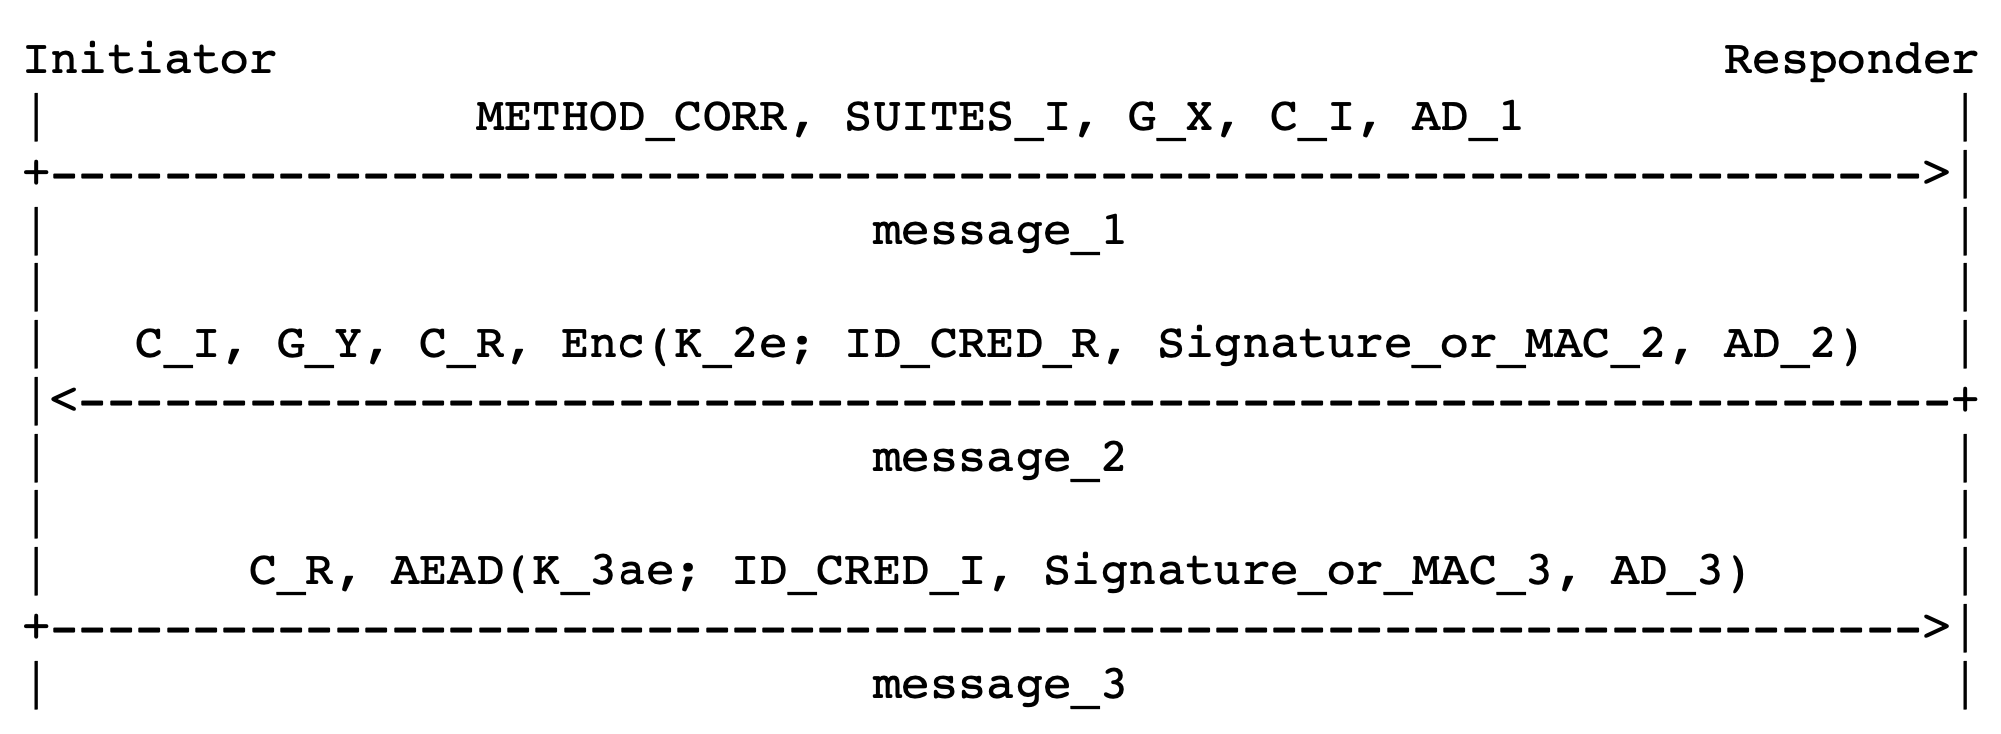
\includegraphics[scale=0.3]{Images/asym.png}
\caption{A template for the asymmetric key methods of EDHOC}
\end{figure}

\subsection{Background, comparison with~\cite{DBLP:conf/secsr/BruniJPS18}}
The first version of \mEdhoc was proposed in March 2016 to a working group investigating lightweight authenticated key exchange protocols [\mcneed]. There has been a focus on formally verifying that the protocol satisfies the properties expected of it right from the beginning. 

The 2018 work~\cite{DBLP:conf/secsr/BruniJPS18} by Bruni et al performed a formal verification of version 08 [\url{https://tools.ietf.org/html/draft-selander-ace-cose-ecdhe-08} \mcfix] of \mEdhoc. The protocol and properties are modelled and verified in the \mProverif tool. This version of the protocol belongs to the \mSigmaI family of protocols, and has two modes -- one with asymmetric keys, and one with pre-shared symmetric keys (PSK). Bruni et al showed that this version satisfies the requisite properties of identity protection, (perfect forward) secrecy of data, and strong authentication, upon completion of the protocol.

\mEdhoc has undergone a lot of change since version 08, as will be described in the following sections, and the formal verification of the current version, therefore, is a worthwhile exercise.

\subsection{Comparison with \mOptls and \mNoise}
\vnote{Would this perhaps be better served by putting it in related work?}


\section{Methods and features of \mEdhoc}\label{sec:methods}

\subsection{Fundamental components of \mEdhoc}
\subsubsection{\mCose}
\mCbor is a data format designed for small code size and small message size. The \mCbor Object Signing and Encryption (\mCose) protocol is used to create and process signatures, MACs, and encryption using CBOR. 

A \mCose object contains bitstrings corresponding to protected parameters (which ought to be cryptographically protected), unprotected parameter, and the payload to be signed. This can be signed/encrypted/MACed, to obtain a resultant \mCose object containing the bitstring corresponding to the operation. The respective algorithms may also be fed some externally supplied data, which is carried along with the \mCose object, but is not part of it. \mEdhoc only uses the signature and encryption objects of \mCose. For encryptions, \mCose supports two different methods -- one where the recipient is not needed because the key is known implicitly, and one for all other cases. \mEdhoc only uses the former. 

A \mCoseEncrypt structure as used in \mEdhoc is a \mCbor array with a text field which contains the string ``Encrypt0'' to denote the use of the method with implicit recipient, a field for protected data, a field for externally supplied application data, and a field for ciphertext. All these fields store the corresponding bitstrings.

\subsubsection{\mAead}
Authenticated encryption with associated data, or \mAead, is an authenticated encryption operation. The algorithm takes in a key, a unique nonce, a plaintext, and some associated data, and outputs a ciphertext. The plaintext is both authenticated and encrypted, while the associated data is merely authenticated. The ciphertext is at least as long as the plaintext. When the plaintext is empty, the \mAead algorithm acts as a MAC on the associated data. 

The associated data is used to protect information that needs to be authenticated, but does not need to be kept confidential. It might be desirable to authenticate this information, although it must be left unencrypted to allow the system to function properly. Authentication is provided without copying the data into the plaintext.

\subsubsection{Key derivation function (KDF)}
Perhaps the most important building block for \mEdhoc is the key derivation function based on \mHkdf [\mcneed], which is used to generate the pseudorandom strings and keys for the encryption operations in the communicated messages. The pseudorandom strings (\mPRKtwo and \mPRKthree) are derived using the \mHkdf-Extract function, while the keys are generated using the \mHkdf-Expand function. Both these functions are based on \mHmac [\mcneed], which is a hashing system for message authentication.

The \mHkdf-Extract function is run with a salt and some input keying material (IKM) as input. It produces as output a pseudorandom string. For the \mPskPsk method alone, the salt is the key pre-shared between the initiator and the responder, while for the other methods, it is empty. The IKM for all \mEdhoc methods is the ECDH shared secret \mGxy.

In order to generate keys for the various encryptions, the \mHkdf-Expand function is used. This is run with a pseudorandom string, an info string, and the length of the output keying material (OKM) as input. The pseudorandom string is generated using \mHkdf-Extract as above. The info string contains details of the \mAead encryption algorithm used, length of the OKM, and the transaction hash as used for the specific method (a detailed discussion follows, for each method). In case the length $l$ of the OKM is shorter than that of the transaction hash, the OKM is obtained by taking the first $l$ bits of the result of running \mHmac on the pseudorandom string, and a concatenation of 0x01 and the info strings.

We now discuss each of the \mEdhoc methods in detail in the next few sections.

\subsection{\mPskPsk method}
In this method, the initiator and responder are assumed to have a pre-shared key which is secret to them, and can be retrieved by the responder using a public part of the first message (\mIDPSK). This method corresponds to the symmetric key method of \mEdhoc v08. 

In the first message, the initiator sends a message consisting of the method name, the cipher suites ranked in order of preference, the initiator's ephemeral key (\mGx), their connection identifier (\mCi), the \mIDPSK identifier, and (optional) auxiliary data (\mADone). The responder, upon receipt of this message, must verify that the selected cipher suite is supported,  and pass \mADone to the security application which needs it. If any verification step fails, the initiator sends an EDHOC error message back, and the protocol aborts.

The second message, sent by the responder, is composed of \mCi, the responder's ephemeral key \mGy, their connection identifier \mCr, and a \mCose object. This contains as external data the transaction hash of the first message (\mTHtwo), along with an \mAead encryption of the (optional) auxiliary data \mADtwo. The key used for this (\mKtwo) is derived using the EDHOC key derivation function with \mTHtwo and the pseudorandom string \mPRKtwo as input, while the associated data for the \mAead encryption is constructed by concatenating a constant string, plaintext \mhplain, and \mTHtwo. Recall that \mPRKtwo is constructed by running \mHkdf-Extract using the pre-shared key as salt. 

The initiator, upon receipt of this message, sends back \mCr, followed by a \mCose object containing an \mAead encryption of auxiliary data \mADthree, along with the transaction hash of the second message (\mTHthree) as external data. As earlier, the key used is derived by supplying \mTHthree and \mPRKthree as input to the KDF, and the associated data obtained by concatenating the constant string, plaintext \mhplain, and \mTHthree. An abstract description is shown in Figure~\ref{fig:edhocpsk}.

\vnote{Figure numbers don't square up, check class file guidelines!}

\begin{figure}[!h]\label{fig:edhocpsk}
\centering
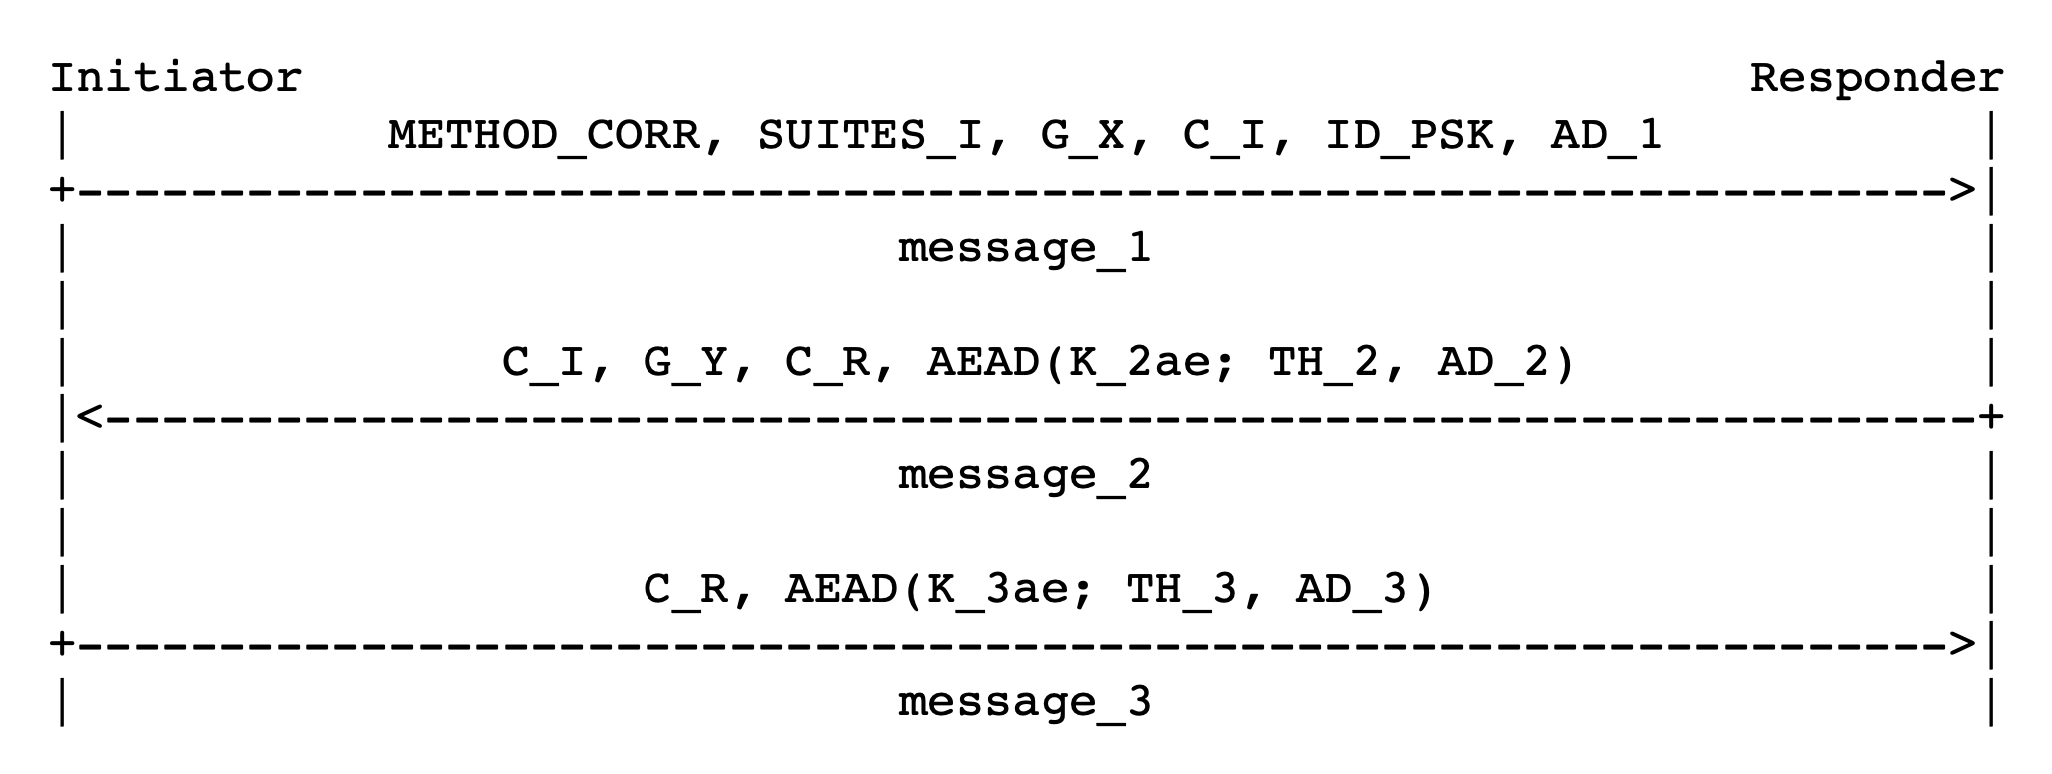
\includegraphics[scale=0.3]{Images/psk.png}
\caption{The PSK-PSK method of EDHOC}
\end{figure}

\subsection{\mStat-based methods}
\mEdhoc allows for three \mStat-based methods -- two where only one participant has a static Diffie-Hellman key (while the other uses signatures), and one where both do. 

In the first message, the initiator includes an identifier for the method, a preference-ordered list of cipher suites, their ephemeral key \mGx, their connection identifier \mCi, and some optional plaintext \mADone. This message is common to all the four methods below involving asymmetric keys. 

The responder, upon receipt, verifies the cipher suites, passes any \mADone to the application that needs it, and proceeds to construct and send the second message. This message contains (not necessarily all of) \mCi, \mGy, \mCr, and an encrypted term. The initiator, upon getting this message, sends out a message containing an encrypted term. Depending on the methods being run by the initiator and responder, the exact contents of these messages may vary. We will now describe each of these methods and the second and third messages therein in detail.

\subsubsection{\mSigStat}
The initiator runs a \mSigma-based method, with signatures, while the responder operates with a static Diffie-Hellman key and MACs. Since this method is one where the responder runs \mStat, in the second message, \mCi is omitted. The encrypted term for the second message is constructed as follows. 

First, we build the \mCose object that is the inner MAC, since the responder runs \mStat. The protected part of this object is an identifier for retrieving the responder's public authentication key \mCredr. The externally supplied data is the transaction hash \mTHtwo of the first message and \mGy,  the responder's public authentication key \mCredr, and (optional) auxiliary data \mADtwo. The key used for the encryption is the output of the KDF on being fed as input the pseudorandom string \mPRKthree and \mTHtwo. The resulting encrypted object is now referred to as the ciphertext \mMactwo. 

For the outer encryption object, we consider the plaintext formed by concatenating the bitstrings corresponding to the identifier for \mCredr, \mMactwo, and \mADtwo (if any). The encryption is obtained by performing an \mXor operation on this plaintext with the key \mKtwo, which is obtained by using the KDF on \mPRKtwo and the transaction hash \mTHtwo. The responder therefore sends to the initiator \mGy, \mCr, and this \mCose encryption object as the second message.

The initiator responds with the third message, consisting of \mCr, and an encrypted object. Here, again, we first build the inner \mCose object. This process is analogous to that employed by the responder for the second message. The \mCose object has as protected data an identifier for retrieving the initiator's public authentication key \mCredi. The externally supplied data is the transaction hash \mTHthree of the second message and \mTHtwo,  the initator's public authentication key \mCredi, and (optional) auxiliary data \mADthree. The key used is obtained by inputing the pseudorandom string \mPRKfour and \mTHthree. The resulting encrypted object is now referred to as the ciphertext \mMacthree. 

Since the initiator is running \mSig, this \mCose object needs to be signed. To the signing algorithm, the initiator sends as protected data the identifier for retrieving \mCredi, as external data the concatenation of \mTHthree, \mCredi, and any \mADthree, and the payload \mMacthree. This is signed using the private authentication key of the Initiator.  

We now construct the encryption for the third message, by passing to an \mAead encryption algorithm a \mCose object with no protected data, external data \mTHthree, and a plaintext obtained by concatenating the identifier for retrieving \mCredi, the signed object described above, and \mADthree. The key used for encryption is \mKthree, obtained by running the KDF on the pseudorandom string \mPRKthree and \mTHthree. Thus, the message sent by the initiator to the responder in the third step is \mCr accompanied by this encrypted object.

\subsubsection{\mStatStat}
In this method, both the initiator and the responder run the \mStat method. The responder's message looks exactly the same as in the previous subsection, for \mSigStat. The initiator's message, however, is not signed anymore, since the initiator too is running the \mStat method. Thus, we skip the signature process in the steps described above, and instead of passing a signed object to the \mAead encryption algorithm, we pass \mMacthree itself. Everything else stays the same as earlier.

\subsubsection{\mStatSig}
Here, the responder runs the \mSig method, while the initiator runs the \mStat method. Thus, the second message, sent by the responder to the initiator needs an extra layer of signing. Once \mMactwo has been constructed, as in the methods where the responder runs \mStat, the responder runs the signature algorithm with a \mCose object. This object has the identifier for \mCredr as protected data, a concatenation of \mTHtwo, \mCredr, and \mADtwo as external data, and the payload \mMactwo. This is signed using the responder's private authentication key.

The outer encryption object is constructed by considering a plaintext consisting of \mCredr, this signed object (instead of \mMactwo, as was the case when the responder ran the \mStat method), and \mADtwo. \mKtwo is generated the same way as earlier, and the responder sends \mGy, \mCr, and this encrypted object to the initiator as the second message.

Since the initiator is running the \mStat method, there is no change in the third message from the previous case. There is no signature, and only \mMacthree is encrypted via \mAead.

\subsection{\mSigSig method}
In this method, both parties run the \mSig method, and therefore, both the second and third messages need to be signed before being encrypted via \mAead. The second message looks like the one from the \mSigStat method described above, while the third looks like the one from the \mStatSig method.


\vnote{Need to insert tikZ figures}

\subsection{Deriving an OSCORE context}
\mEdhoc is often used to set up parameters for \mOscore. In this case, the parties make sure that the connection identifiers are distinct, i.e. $\mCredi \neq \mCredr$, since these are used as \mOscore sender IDs. If the initiator plays the role of the CoAP client, and the responder the role of the CoAP server, the client gets the sender ID \mCredr and the server the ID \mCredi (the identifiers are swapped). The \mAead and hash algorithms for \mOscore stay the same as those used for the selected cipher suite in \mEdhoc, while the master secret for \mOscore is derived using the key length of the \mAead algorithm of \mEdhoc. 

\subsection{Expected security properties}



%-------------------------------------------------------------------------- sec
\section{Formalization and results}
\label{sec:formalization}
\hl{Alessandro}
% !TEX root =  main.tex
 
Next we describe our approach towards formalizing the \mEdhoc{} protocol. We use the
symbolic (Dolev-Yao) model for verification, with \mTamarin{} for tool support.
%
The next three subsections describe our threat model, briefly present the
\mTamarin{} tool, and our modeling choices.
%
Finally, we present the properties that we proved in this effort.

 
\subsection{Threat Model}\label{sec:threat-model}
 
We verify \mEdhoc{} in the symbolic Dolev-Yao model: as customary in this style of
modeling, we assume all cryptographic primitives to be ``perfect'', and hence
only allow the attacker to encrypt and decrypt messages when they know the key,
and exclude hash collisions, for example; the attacker is in control of the
communication channel, and can interact with unbounded sessions of the protocol,
dropping, injecting and modifying messages at their liking.

One important point of the modeling is that we allow the attacker to impersonate
dishonest and/or compromised endpoints, by revealing their long-term and session
key material at any given point.
%
Conversely, we say that a party is honest if they never reveal their
long-term key or session key material.

Another important point is to define what the key material is.
    \mEdhoc{} does not result in an explicit session key, but a cryptographic
    state from which keys for \mOscore{} can be derived using \mHkdf.
    As will be seen below, depending on how the key material is defined, the
    different methods will have different authentication properties.
    In particular, all methods except those where the initiator uses the
    \mStat{} method provide a stronger form of authentication (injective
    agreement) for the initator.

 
\subsection{Desired Properties}
\label{sec:desired-properties}
 
Next we list the properties that will be considered during verification.
\knote{The title should be "verified properties" or "considered properties" or
    similar. "desired" requires us to specify who think they are desired and
    give rationale for why the are desired.  Also, one of the points of the
    paper is that without more specific goals for EDHOC, it is not clear what
constitutes desirable.}

 
\subsubsection{Secrecy}
\knote{Please add a dot at the end of all subsubsections and paragraphs (llncs
guidelines)}
We say that \mEdhoc{} satisfies secrecy of the established session key $sk$
between two honest parties $A$ and $B$ if, for any run of the protocol $A$ and
$B$, the attacker does not get to know $sk$.
%
The attacker may passively observe---and actively interfere with---the
communication, and run any number of sessions with $A$ and $B$, in either role,
concurrently or otherwise.

 
\subsubsection{Authentication}
To define \mEdhoc{}'s authentication properties we make use of Lowe's definition
of \emph{injective agreement}~\cite{DBLP:conf/csfw/Lowe97a}:
\knote{Maybe we don't need to quote the definition and could paraphrase it in a
shorter form to save space.}
\begin{quote}
  ``We say that a protocol guarantees to an initiator $A$ [injective] agreement
  with a responder $B$ on a set of data items $ds$ if, whenever $A$ (acting as
  initiator) completes a run of the protocol, apparently with responder $B$,
  then $B$ has previously been running the protocol, apparently with $A$, and
  $B$ was acting as responder in his run, and the two agents agreed on the data
  values corresponding to all the variables in $ds$, and each such run of $A$
  corresponds to a unique run of $B$.''
\end{quote}
%
We say that \mEdhoc{} in method $m$ satisfies \emph{explicit authentication} for
the initiator $A$ with a responder $B$, if injective agreement holds for $A$
with $B$ on the session key $sk$, when running method $m$.
%
The corresponding definition for the responder is analogous.
%
If both parties obtain explicit authentication we refer to it as mutual explicit
authentication or simply explicit authentication when it is clear from the
context.

A party obtains the explicit authentication guarantee when both parties agree
on the session key (and other parameters), when the party completes the protocol
run.
%
It turned out, however, that explicit authentication does not hold for all
\mEdhoc{} methods, in which cases we prove \emph{implicit authentication} as
defined in~\cite{DBLP:journals/iacr/GuilhemFW19}.
%
In a nutshell, a protocol satisfies \emph{implicit authentication} if the
initiator and responder agree on the session key \emph{only after} a successful
execution of the protocol.
%
That is, authentication happens only implicitly, as there is no confirmation to
the initiator that the responder has computed the same session key.
%
More precisely, we adapt the definition of~\cite{DBLP:journals/iacr/GuilhemFW19}
to the symbolic model, and we prove that if an initiator $A$ and a responder $B$
complete the protocol deriving the same session key, then $A$ believes she is
talking to $B$ and $B$ believes he is talking to $A$.

 
\subsubsection{Session Independence}
A protocol satisfies session independence if knowing a session key does
not give the attacker any information about other sessions.  To model session
key independence of \mEdhoc, we allow leakage of session keys, and additionally
check security only of those sessions for which the session keys have not been
directly revealed to the attacker.

 
\subsubsection{Perfect Forward Secrecy} (PFS) A protocol satisfies perfect forward
secrecy if, for any run of the protocol in which the initiator and the responder
agree on a session key $sk$, the attacker does not learn $sk$, even when the
long-term keys are revealed after the session is completed.

 
\subsubsection{Key-Compromise Impersonation} (KCI) This property takes the perspective of one
of the endpoints of the protocol, say Alice running a session with Bob. A
protocol is secure under KCI if Alice can still establish a secure session with
Bob, even though Alice's keys are compromised at any time, and Bob's key
material is not leaked until the end of the session.

 
\subsubsection{Post-Compromise Security} (PCS) A protocol that has
\emph{post-compromise security} (following definitions in~\cite{cohn2016post})
is capable of establishing a secure session even after one of the parties has
been compromised. Cohn-Cordon et al.~\cite{cohn2016post} presents two notions of
PCS, namely weak and strong PCS: here we focus on the latter.
%
A protocol guarantees \emph{weak PCS} if secrecy of any session key $sk$ holds
between the initiator and the responder, even if the run of the protocol that
established $sk$ happens after a \emph{limited compromise}, where the key
material is not leaked, but the attacker is capable of impersonating both
parties (i.e. has the ability to perform all cryptographic operations using the
initiator's and responder's long term keys, but has not access to the long term
keys).

 
\subsection{\mTamarin{}}
\label{sec:tamarin}
 
We chose \mTamarin{} to model and verify \mEdhoc{} in the Symbolic model.
%
\mTamarin{} is an interactive verification tool based on multi-set rewriting rules
with event annotations, which allows the user to check Linear Temporal Logic
(LTL) formulas on these models.
%
Multi-set rewrite rules with events take the form $ l \ifarrow[e] r $,
where $l$ and $r$ are multi-sets of facts, and $e$ is a multi-set of events.
Facts are $n$-ary predicates over a term algebra, which defines a set of function
symbols $\mathcal F$, variables $\mathcal V$ and names $\mathcal N$. \mTamarin{}
checks equality of these terms under an equational theory $E$. For example,
one can write $ dec(enc(x,y),y) =_E x $
to denote that symmetric decryption reverses the encryption operation under this theory.
All operations on terms are defined under $E$, hence we omit the
subscript from now on as the equational theory is fixed per model.

 
\subsubsection{Semantics and Built-ins} \phantom{} \mTamarin{} states
$S$, $S'$ are multisets of facts, and a semantic transition $S \semarrow[E] S'$
occurs if there is a rule $l \ifarrow[e] r$ and a substitution $\sigma$ such
that $S \supseteq \sigma(l)$ and $S' = S \setminus \sigma(l) \uplus \sigma(r)$
and $E = \sigma(e)$.

There are a few more details, such as persistent facts that are denoted by a $!$
and are never removed from the state.
%
The sorts fresh (denoted by $\sim$) and public (denoted by $\$$) denote fresh
constants and public values known to the attacker respectively, and are both
sub-sorts of a base sort.
%
Finally, \mTamarin{} has some built-in predicates ($\mIn,
\mOut$ to represent input and output of messages with the attacker,
and
$\mFr$ to denote a fresh constant created in the current rule, among
others), rules and equations that represent the attacker's knowledge
and standard equational theories in the symbolic model,
which we present later.

\anote{This can go, I make a shorter note later:\\
{Notational conventions} In the remainder of this section we present
\mTamarin{} code as it appears in the models that we verify, in the style of
literate programming.  Whenever possible we match the style of the protocol
diagrams in Section~\ref{sec:edhoc} and the naming convention of the \mEdhoc{}
\mSpec~\cite{selander-lake-edhoc-01}, so that each element of the model is
traceable to the standard.  There are a few exceptions to this, most notably
some variable names that we introduce for the sake of the \mTamarin{} model and are
not present in the original \mSpec{}, which will appear in \mT{camelCase}, and
the syntax for Diffie-Hellman exponentiation which is specific to \mTamarin{}.
We also use \mT{xx} to name the ephemeral key for the initiator (resp. \mT{yy}
for the responder) as to avoid confusion with \mTamarin's builtin variable
names \mT{x} and \mT{y}.}

 
\subsubsection{Protocol Rules and Equations}
\mTamarin{} allows users to define new function symbols and equational theories.
These user defined objects are then translated by \mTamarin{} into rewrite
rules, which are added to the set of considered rules during verification.
For example, in our model we have a symbol to denote authenticated encryption and
hence \mTamarin{} produces the rule:
%
\begin{lstlisting}
[!KU(k), !KU(m), !KU(ad), !KU(al)] --> [!KU(aeadEncrypt(k, m, ad, al))]
\end{lstlisting}
%
to denote that if the attacker knows a key \mT{k}, a message \mT{m}, the
authenticated data \mT{ad}, and an algorithm \mT{al}, then they can construct
the encryption using these parameters, hence get to know the message
\lstinline{aeadEncrypt(k, m, ad, al)}.

In our model we introduce a theory for authenticated encryption, and make use of
the built-in theories of exclusive-or and Diffie-Hellman operations.
%
Authenticated encryption, which is encryption with authentication data as
detailed in~\cite{aead}, has the following two equations:
\begin{lstlisting}
aeadDecrypt(k, aeadEncrypt(k, m, ad, al), ad, al) = m
decrypt(k, aeadEncrypt(k, m, ad, al), al) = m
\end{lstlisting}
With the first rule we allow the protocol to decrypt the message \mT{m} if the
encryption has matching key \mT{k}, authenticated data \mT{ad}, and uses the
same algorithm \mT{al}.
%
The second rule allows the attacker to decrypt the message \mT{m} with the key
\mT{k} and without the authenticated data \mT{ad}, and hence skip the check.

The built-in theories for XOR and Diffie-Hellman are a fair bit more complex
than authenticated encryption, hence we refer to the original
papers~\cite{DBLP:conf/csfw/DreierHRS18,DBLP:conf/csfw/SchmidtMCB12}
for a full reference.
%
Suffices to say that the XOR theory introduces the symbol \mT{XOR}, for
expressing XOR operations \mT{x} $\oplus$ \mT{y}, plus the necessary equational theory
including associativity, commutativity, and inverse.
%
The theory for Diffie-Hellman introduces exponentiation \mT{g^y} and product of
exponents \mT{x * y} as a built-in symbols in the language, plus the necessary equational
theory of associativity, commutativity, distributivity of exponentiation with
product, and inverse.

 
\subsubsection{Syntactic Sugar} In the following presentation we use some syntactic
sugar, which is necessary to understand to look at the concrete rules. First is
the use of let bindings (\mT{let ... in}), which are series of
definitions of patterns which are substituted in the rest of the rule. Another
prominent feature is the use of tuples (\mT{<t1, ..., tn>}) which are a
built-in concept in \mTamarin.

 
\subsection{Modeling \mEdhoc{}}
 
In this section we detail the modeling choices that we have made for this formal
verification effort.
%
We model the five different methods of \mEdhoc{} from a single specification
using the M4 macro language to derive all valid combinations: \mPskPsk,
\mSigSig, \mSigStat, \mStatSig{} and \mStatStat.
%
Whenever possible we adhere with the variable names present in the standard and
in Section~\ref{sec:edhoc}. There are a few exceptions: we present in
\mT{camelCase} those names introduced with the modeling, and we use \mT{xx} and
\mT{yy} for the ephemeral keys, to avoid name clashes.
%
\anote{Do we need this: Other parameters to the model include the optional data of the \mEdhoc{}
specification, that is, the connection identifiers \mCi{} and \mCr{}, and
the authenticated data \mADone, \mADtwo{} and \mADthree.}
%
To keep the presentation brief, we only present the \mStatSig{} mode, as it
shows both asymmetric modes at the same time. The PSK case can be found in the
appendix and the full code at the GitHub repository~\cite{edhocTamarinRepo}.
\anote{Fix: give a dropbox link instead of the repo}
% - Explain details of model, which properties we have modeled, how,
% which trade-offs were made and why.
 
\subsubsection{General Setup}
\vnote{Section name doesn't appear here! Needs some text before the rule.}
\begin{lstlisting}
rule registerLTK_SIG:
 [Fr(~ltk)] --[ UniqLTK($A, ~ltk) ]->
  [!LTK_SIG($A, ~ltk), !PK_SIG($A, pk(~ltk)), Out(<!<$A, pk(~ltk)>!>)]
rule registerLTK_STAT:
 [Fr(~ltk)] --[ UniqLTK($A, 'g'^~ltk) ]->
  [!LTK_STAT($A, ~ltk), !PK_STAT($A, 'g'^~ltk), Out(<!<$A, 'g'^~ltk>!>)]
\end{lstlisting}

These rules express the registering of the long term keys for the \mSig{} and
\mStat{} methods, respectively.
%
\mT{registerLTK_SIG} and \mT{registerLTK_STAT} register a public key (for
signing and encrypting, respectively) that are tied to the identity of an agent
\mT{A}. A similar rule \mT{registerLTK_PSK} registers symmetric keys for pairs
of agents.
%
The event \mT{UniqLTK} marks that the long term key is unique for each
agent.
% or pair of agents, as enforced by the following restriction:
% \begin{lstlisting}
% restriction uniqLTKs:
%     "All id k1 k2 #i #j. (UniqLTK(id, k1)@i & UniqLTK(id, k2)@j) ==> k1 = k2"
% \end{lstlisting}
This models that there is an external mechanism ensuring that the
long term keys are bound to the correct identity, e.g., a certificate authority,
and that the attacker cannot register new public keys for an existing identity.

In our model we introduce specific rules to give the attacker access to
long-term keys, session keys and the cryptographic interface of the device.
\begin{lstlisting}
rule revealLTK_SIG: [!LTK_SIG($A, ~ltk)] --[LTKRev($A)]-> [Out(~ltk)]
rule revealLTK_STAT: [!LTK_STAT($A, ~ltk)] --[LTKRev($A)]-> [Out(~ltk)]
rule revealSessionKeyI: [CommitI(tid, u, v, sk)] --[SKRev(sk)]-> [Out(sk)]
rule revealSessionKeyR: [CommitR(tid, u, v, sk)] --[SKRev(sk)]-> [Out(sk)]
rule forge_SIG: [!LTK_SIG($A, ~ltk), In(xx)] --[TEE($A)]-> [Out(sign(xx, ~ltk))]
rule exp_STAT: [!LTK_STAT($A, ~ltk), In('g'^x)] --[TEE($A)]-> [Out(('g'^x)^~ltk)]
\end{lstlisting}
These rules allow to check Perfect Forward Secrecy, Key Compromise Impersonation
and (weak) Post Compromise Security as defined in Section~\ref{sec:desired-properties},
by giving the attacker the ability to access to long term and session keys, or
to the cryptographic interface, at the appropriate time.

\subsubsection{Modeling Choices}

We model each method of the protocol with four rules: \mT{I1}, \mT{R2}, \mT{I3}
and \mT{R4} (with the current method suffixed to the rule name) represent each
step of the protocol as run by the Initiator \mT{I} and the responder \mT{R}.
Each rule can be traced back to the diagrams of Figure~\ref{fig:edhocsigstat}
and Figure~\ref{fig:edhocstatsig}.
%
The full code can be found at the appendix, however there are a few important
modeling details to discuss.

The way \mT{m1} is constructed differs slightly from the specification. In
particular, the \emph{method} field is divided into two fields representing the
method for the initiator and the responder, the connection identifier is omitted
and the ciphersuite is represented by the public variable
\mT{$cSUITES0} (known to the attacker). We plan to introduce the connection
identifier \mCi in our ongoing verification effort, whereas the other two are
modeling choices that do not affect the behaviour of the model.

We model the XOR encryption of \mT{CIPHERTEXT_2} with the key \mT{K_2e} as to
allow recovering of part of the key for known plaintext.
%
Hence \mT{CIPHERTEXT_2} is not a direct XOR ``encryption'' in the model, but
rather a tuple where each field is XORed with a half-key expansion (\mT{K_2e_1}
and \mT{K_2e_2}).

We use the facts such as \mT{StI1_PSK_PSK($U, ~ltk, $V, ~xx, m1, ~tid)} %
to save the internal state for the remainder of the initiator's protocol (here
for the \mPskPsk{} case).

We mark different steps of the protocol with \mT{Running} and \mT{Commit}
events. These events are used to mark that one of the party has started or
completed the protocol.
%
For example, the event \mT{ExpRunningR(~tid, $V, exp_sk)} %
marks that the responder has started the protocol and they currently believe
that \mT{exp_sk} is the session key.
%
Other events like \mT{ExpCommitI(~tid, $U, $V, exp_sk)} %
and \mT{CommitI(~tid, $U, $V, imp_sk)} mark the completion of the protocol for
the initiator, and will be used later for verifying explicit and implicit
authentication, respectively.  The difference is the choice of key material on
which we check authentication (\mT{exp_sk} vs \mT{imp_sk}). In the case of the
\mSig{} method, as above, these keys are the same, but there will be a crucial
difference when the initiator runs the \mStat{} method.

\emph{Implicit authentication} differs from explicit authentication when the
Initiator runs the static method: on \mT{imp_sk} the semi-static key \mGiy{} is
present, whereas \mT{exp_sk} does not include it for injective agreement.
%
The reason for this is that, when sending message 2, the responder does not yet
know the identity of the initiator, hence an active attacker can interfere with
the protocol in such a way that the two parties do not agree on the semi-static
key \mGiy{} until after the end of the protocol, when the responder starts using
the derived key material with the initiator.
%
What happens after \mEdhoc{} completes is beyond the scope of our study, hence
we have left this part out of the modeling and only focus on the key material
that both parties agree on.
%
In future work, it will be interesting to see the interaction of \mEdhoc{} with
\mOscore{} which can use \mEdhoc{}'s keys.

 
\subsection{Properties}
\label{sec:properties}
 \anote{TODO: rework the text here}
\knote{Vaishnavi found out that appendices are included in the page count after
    all. We therefore decided to create a tech report with the full text instead
    and put that in drop box with the model. Then this paper refers to the tech
    report. So, put the parts that won't fit into the page limit into an annex,
    but cite it as a reference to the tech report, not the annex.
}
In this section we present the properties that we have shown for \mEdhoc, and
show the lemmas that verify them. We refer to
Section~\ref{sec:desired-properties} for a full explanation of the properties
that we check. Here we focus on their formalization into \mTamarin{} lemmas.

 
\subsubsection{Explicit Authentication}

We model explicit authentication between the initiator and the
responder.
%
For this lemma, we use the events \mT{ExpCommitI} and
\mT{ExpRunningR}, and show that there is injective agreement
between the two events on the parameters \mT{tidI},
\mT{v} and the session key material \mT{expSk} (note
that the session key material changes between the different \mEdhoc{}
methods).

Additionally, we require that injective agreement must hold only when
no long term key material for the two parties has been revealed before
the end of the protocol.
%
This is achieved by the main disjunction in lines 5-10 on the right of
the implication, requiring to reveal the long term keys (i.e. one of
the three \mT{LtkRev} events must trigger) if the responder has
not been running a matching session with the initiator.

\knote{We can remove the line "all-traces" from all listings to save space.
It is Tamarin's default. One only have to add "exists-trace" explicitly.}

\begin{lstlisting}
lemma authInjAgreeGuaranteeForI:
    all-traces
    "All tidI u v expSk #i.
         (ExpCommitI(tidI, u, v, expSk)@i
	     & (All #j m1. I1(tidI, u, v, m1) @ j ==> (All #k. TEE(u)@k ==> k < j) & (All #k. TEE(v)@k ==> k < j))
         & (All tidR #j m1 m2. R2(tidR, v, m1, m2) @ j ==> (All #k. TEE(u)@k ==> k < j) & (All #k. TEE(v)@k ==> k < j)))
          ==>
         ( ( (Ex tidR #j. ExpRunningR(tidR, v, expSk)@j & #j < #i)
           & not(Ex tidI2 u2 v2 #i2. ExpCommitI(tidI2, u2, v2, expSk)@i2 & not(#i = #i2) ) )
         | (Ex #j. LTKRev(v)@j & #j < #i) )"
\end{lstlisting}

Note that this property \emph{does not hold when} the initiator is
running the \mStat{} method.
%
For that case we need to prove implicit authentication, as detailed in
the next section.

Similarly to the previous lemma, we require that injective agreement also holds
in the reverse direction:

\begin{lstlisting}
lemma authInjAgreeGuaranteeForR:
    all-traces
    "All tidR u v sk #i.
         (CommitR(tidR, u, v, sk)@i
	     & (All tidI #j m1. I1(tidI, u, v, m1) @ j ==> (All #k. TEE(u)@k ==> k < j) & (All #k. TEE(v)@k ==> k < j))
         & (All #j m1 m2. R2(tidR, v, m1, m2) @ j ==> (All #k. TEE(u)@k ==> k < j) & (All #k. TEE(v)@k ==> k < j)) )
         ==>
         ( ( (Ex tidI #j. ExpRunningI(tidI, u, v, sk)@j & #j < #i)
           & not(Ex tidR2 u2 v2 #i2. ExpCommitR(tidR2, u2, v2, sk)@i2 & not(#i = #i2)) )
         | (Ex #j. LTKRev(u)@j & #j < #i) )"
\end{lstlisting}

As the explicit and implicit authentication always correspond for the
responder authenticating with the initiator, here we do not need the
additional \mT{Exp} prefix to the running and commit events
(\mT{CommitI} and \mT{CommitR} respectively).

 
\subsubsection{Implicit Authentication}

The following lemma proves implicit authentication:
\begin{lstlisting}
lemma authGIYImplicitAuthGuaranteeForI:
    all-traces
    "All tidI u v impSk #i.
         CommitI(tidI, u, v, impSk)@i ==>
         ( ( (All tidR u2 v2 #j. CommitR(tidR, u2, v2, impSk)@j ==>
                (u = u2  &  v = v2)
             )
           &
             (not Ex #k. K(impSk)@k)
           &
             (not( Ex tidR u v #j tidR2 u2 v2 #j2.
                      ( CommitR(tidR,  u,  v,  impSk)@j
                      & CommitR(tidR2, u2, v2, impSk)@j2
                      & not(#j = #j2)
                      )
                 )
             )
           )
         | (Ex #k. LTKRev(u)@k) | (Ex #k. TEE(u)@k)
         | (Ex #k. LTKRev(v)@k) | (Ex #k. TEE(v)@k)
         )
         "
\end{lstlisting}

As opposed to lemma \mT{authInjAgreeGuaranteeForI}, here we prove that the two
parties implicitly authenticate on the keys \mT{impSk}. %
In this lemma we show that if any two parties (\mT{u} and \mT{v2} here) complete
a run of the protocol, and \mT{u} believes she is talking to \mT{v} and \mT{v2}
believes he is talking to \mT{u2}, then their identities match (that is,
\mT{u = u2} and \mT{v = v2}). Furthermore there is an injective correspondence
between the \mT{CommitI} and \mT{CommitR} events, and the attacker does not
learn the session key material.

 
\subsubsection{Secrecy, Forward Secrecy and Session Key Independence}

Finally, we prove secrecy of session keys, perfect forward secrecy
(PFS) and session key independence.
%
All these properties are validated by a unique lemma for each method,
as secrecy is a strictly weaker property than PFS (and hence follows
directly), and session key independence can be proven along PFS.
%
This is done by allowing the revelation of long term keys after either
the initiator or the responder have completed the protocol, and by
allowing to reveal the session keys.
%
It still holds that the session keys are secret for all the other runs
of the protocol.

We present the lemma for the \mSigStat{} method:
\begin{lstlisting}
  lemma secrecyPFSGIYSessionKey:
        all-traces
        "(All tid u v sk #i #j. (K(sk)@i & CommitI(tid, u, v, sk)@j) ==>
            ((Ex #l. LTKRev(u)@l & #l < #j) | (Ex #l. LTKRev(v)@l & #l < #j) | (Ex #l. SKRev(sk)@l) | (Ex w #l. TEE(w)@l))
         )
         &
         (All tid u v sk #i #j. (K(sk)@i & CommitR(tid, u, v, sk)@j) ==>
            ((Ex #l. LTKRev(u)@l & #l < #j) | (Ex #l. LTKRev(v)@l & #l < #j) | (Ex #l. SKRev(sk)@l) | (Ex w #l. TEE(w)@l))
            )"
\end{lstlisting}

%%% Local Variables:
%%% mode: latex
%%% TeX-master: "main"
%%% End:


%-------------------------------------------------------------------------- sec
\section{Discussion}
\label{sec:discussion}
%-------------------------------------------------------------------------- sub
\subsection{Design Practices}
\label{sec:designPractices}
\knote{Note to self: Long sentences. Not to the point. Revision needed.}
We start with two observations on the design practices, which the \mEdhoc{}
design shares with many other standards specifications.
%
\mPoint{Lack of clear security model}
The first observation is the lack of clearly defined security model.
%
This is common in standardization, and a nuisance for the formal methods
community~\cite{DBLP:conf/ccs/BasinDHRSS18}, who appear to expect industrial
standards, from organizations such as IETF and 3GPP, to be built from a
semi-theoretical framework to meet precise design goals.
\knote{Need to polish this sentence to not offend anyone.}
\vnote{I'm probably not sure whether this paragraph serves any purpose at all. Can be included into the next paragraph, without explicitly saying that the lack of a model is common in standardization or berated by the formal methods community.}
%
Because industrial standards aim to meet the needs of
existing, mixed with envisioned, use-cases, the work has a significant
explorative element.
%
Defining a strict security model from the start is difficult in this setting.
%
In many cases, a security model evolves during the design and is defined
by resistance to the attacks discussed in the process, not by a small set of
precise assumptions and the consequences drawn from those. \vnote{Why not? Should perhaps also make a note of designers being unused to thinking of protocols and models in the formal methods sense.}
%
Even so, the lack of security model in \mEdhoc{} is somewhat troubling in that it does not even discuss general use-cases in its requirements
document~\cite{ietf-lake-reqs-04}.
%
The rationale is instead derived purely from technical aspects of the devices,
communication links and accompanying protocols with which \mEdhoc{} is to be used.
%
No direct consideration is given to the intended uses-cases for the systems
built from these technical components.
%
Because of this, it is unclear which security properties \mEdhoc{} should have.
%
Nonetheless, the \mSpec{} makes a number of detailed claims of properties
the protocol provides (see Section 8.1~\cite{selander-lake-edhoc-01}).
%
The intention may be that, if the academic protocol \mSigma{} is re-used as a
cryptographic core of \mEdhoc, then all the properties listed
in the paper analyzing \mSigma~\cite{DBLP:conf/crypto/CanettiK02} are the
necessary and sufficient ones and can be copied into the \mSpec.
%
(Note: likely the intention is the same for the other reused academic protocols,
but since the \mSpec{} is still work in progress, it is not yet written
down).
%
Section~8.1. states, \emph{"EDHOC inherits its security properties
from the theoretical SIGMA-I"}.
%
Designing a standard specification by re-using existing well-studied academic
components is good practice, but this approach has two problems.
%
First, it is unknown whether the properties provided by the cryptgraphic cores
are suitable for the situations in which \mEdhoc{} is to be used, whether
something is missing, or whether something is unnecessary.
%
The latter should be of concern because of the aim to optimize \mEdhoc{} for
message size. \vnote{Second or third? What is the ``latter'' in a list of three?}
%
Second, \mSigma{} and the other cryptographic cores used by \mEdhoc, are
typically designed for a precise setting with many underlying assumptions.
%
Without spelling those out in the \mSpec, and without showing how
\mEdhoc's adaptations to the cryptographic cores map to the academic protocols
used, such claims are not very informative and may even be misleading.
%

Another concrete example, which we believe is important, is whether distributing
\mEdhoc{} processing across a trusted execution environment (TEE) and a less
trusted part, should be considered in the security model.
%
In our analysis we have chosen not to model such a distribution.
%
This is because we received indications that it was not necessary to consider
reveal of the session state, in particular the ephemeral secret keys when
\mSigma{} cannot protect against such an attack.
\knote{Personal correspondence. Should we include that?}
\vnote{Yes we should, definitely needs a citation of some sort.}
%
This is however only true if one restricts attention to key confidentiality.
%

We believe it would be useful to consider TEEs. \vnote{Unnecessary sentence, follows smoothly from the previous paragraph.}
%
For example, TEE can provide protection against many other threats than
confidentiality.
%
Given that many IoT devices will be deployed in hostile environments there may
be use-cases where it may be acceptable that confidentiality is compromised, but
where impersonation attacks would be dangerous.
%
Further, \mEdhoc{} re-uses cryptographic cores from academic protocols such as
\mSigma{} and \mOptls, which were intentionally designed for a well-defined
security model where compromise of ephemeral keys is less critical than
compromise of long-term keys.
%
Not taking advantage of this seems wasteful.
%
With at least a roughly drawn security model, these considerations would have
surfaced earlier in the standardization process.
%
\textbf{Proposal:} We do not suggest that standard security protocols
necessarily should be built bottom up based on a formal theoretical framework.
%
Doing so would be helpful for subsequent formal verification, but would
likely grind standards to a halt.
%
However, it would be useful to add some justification for claims and the
intended mapping of the cryptographic core to the academic protocol used and
which differences there are.
%
This would greatly help academics to reverse engineer appropriate security
models and verify whether the claims do hold in that model.
%
It would also be useful to capture the intended uses of end-systems on a high
level to learn which security properties are required.
%

\mPoint{Property diversity between methods}
Our second observation is that the five different methods provide very different
security guarantees.
%
Each one is tailored for a specific situation, and the overarching goal of
optimization of message sizes resulted in them providing different guarantees.
%
However, when it comes to implementation and use of the protocol, this shifts the
responsibility of selecting the appropriate version to the user.
%
Should \mEdhoc{} become the protocol of choice for all the IoT applications to
come, it is easy to imagine developers downloading an \mEdhoc{} library and using
it similarly to how \mTls{} is used today.
%
Many developers will assume that \mEdhoc{} provides sufficient security and may
chose method based on performance rather than on security properties.
%
For example, consider a use-case where \mEdhoc{} is run over a near-field
communication radio to derive a token from the derived session key.
%
The token is then to be used at a later point in time.
%
In this case it would be useful that both parties get confirmation that the
other party computed the session key (key confirmation).
%
This property is not achieved by the \mEdhoc{} methods where the initator uses the
\mStat{} method for authentication.
%
Obviously, this can be solved on the application layer, but only if the
developer is aware of the discrepancy.
%

Another aspect showing the usefulness of considering \mEdhoc{} light-weight
use-cases is that, until we pointed it out, the \mSpec{} did not contain
any discussion on the topic of (non)-repudiation.
%
Non-repudiation may be a very useful property for an access control
solution for a nuclear power-plant, whereas it may undesirable for privacy
purposes in coffee vending machine.
%
Such a simple thought experiment would have caught the missing topic.
%
\textbf{Proposal:} There are some use-cases discussed in the LAKE working
group requirements draft~\cite{ietf-lake-reqs-04}.
%
It would, however, be useful to extend the security considerations section in
the \mSpec{} with example use-cases and showing the consequences of
choosing different methods.
%
It would also be helpful to capture and analyze more informal and light-weight
use-cases in the requirements document, to better understand which properties
are needed.
\knote{Adjust the last sentence depending on what happens to the requirements
draft.}

%-------------------------------------------------------------------------- sub
\subsection{Unclear identity management and authentication}
\label{sec:usableSecurity}
\mPoint{Protocol is unclear about what it means by authentication; also, why is
mutual auth required?}
%
The \mSpec{} is unclear about what kind of authentication it aims to achieve.
%
Most importantly, it is not stated whether implicit or explicit authentication
is required, or whether confirmation of the peer's agreement on the \mSid{} or
session key. \vnote{Incomplete sentence?}
%
As our analysis shows, mutual injective agreement on the \mSid{} is achieved
by all methods, except for when the initiator is using the \mStat{} methods.
%
This is because the \mSid{} is unique among sessions (in the symbolic model it
is since the ephemeral keys are fresh and in the computational model they are
fresh with overwhelming probability). \vnote{This note seems unnecessary}
%
Injective agreement provides explicit authentication.
%
In case the initiator uses the \mStat{} method, only implicit authentication
can be achieved.
%
Whether explicit authentication is an important feature for \mEdhoc{} or not, and
whether it violates the requirement on mutual
authentication~\cite{ietf-lake-reqs-04} is difficult to say.
%
Neither does the requirements document~\cite{ietf-lake-reqs-04} provide
intended use cases hinting at what level of authentication is required, nor does
it explain what the more technical term "mutual authentication"
is intended to cover.
%
\textbf{Proposal:}
It would be useful to clarify in the \mSpec{} that different methods provide
different types of authentication and elaborate on in which situations and
implementer should select which method.
%
The latter is important in an industrial standard because it can be expected
that many implementers may otherwise end up with an insecure solution
by select the most efficient method. \vnote{This ties into the previous subsection as well. Perhaps merge the two?}
%

The requirements~\cite{ietf-lake-reqs-04} demand mutual authentication, but
do not provide any rationale, more than that it is expected of IETF protocols
(see Section 3).
%
We observe that if it is acceptable to sacrifice explicit authentication for
some methods to obtain shorter messages, it may also be acceptable for some
use-cases to only provide unilateral authentication and by that reducing the
number of messages to one round-trip.
%
Similar to how \mTls{} is often used, initiator authentication could then be
performed on the \mCoap{} level in the secure \mOscore{} channel.
%
Such a combination of authentications has worked well for many web
use-cases and provides mutual authentication for the application on a system
level.
%
Since few protocols, \mEdhoc{} included, are expected to work in isolation, this
may be a possible approach.
%
\textbf{Proposal:} Without some use-cases or user-stories, it is difficult to
determine whether mutual authentication is an appropriate requirement or whether
a more optimized unilateral authentication solution with possible \mCoap{} level
authentication would be better.
%
We propose considering light-weight use-case analysis to explore this option.
%

\mPoint{not verifying \mIdcredr{} is dangerous}
Section 3.2 of the \mSpec, states that a policy is required restricting the set
of peers an entity is allowed to run \mEdhoc{} with.
%
However, because the initator is not required to verify that the \mIdcredr{}
received in message 2 is the same as the one it intended when sending message 1,
this is insufficient for a general purpose AKE.
%
These small thought example shows why.
%
Assume someone has configured all devices in their home to be in the restricted
set, but that one of the devices $A$ has been compromised.
%
If another device $B$, unaware of the compromise, initiates a connection to a
third device $C$, the compromised device $A$ may interfere.
%
$A$ may respond in $C$ place, which may require blocking the response from $C$.
%
Since $A$ does not check that it is $C$'s identity in message 2, and device $A$
is part of the restricted set, $A$ will complete and accept the \mEdhoc{} run with
device $A$.

\vnote{Naming issues in this example here, check. Some confusion of $A$ and $B$.}
%
The obvious solution is for the initiator to match \mIdcredr{} to the intended
identity.
%
This is yet another example of where a small use-case or user-story uncovers
potential lacks in the \mSpec, and show that it would be a useful addition to
the requirements document~\cite{ietf-lake-reqs-04}.

\vnote{I feel like sections 4.1 and 4.2 together serve to give a rather long-winded rationale for the fact that there the specification a) ill-specifies some security properties, and b) does not root its desirable properties in any use-cases, especially considering that the various methods fulfil different properties. It might be worthwhile to consider editing this part to merge all these sections, with short descriptions of these possible pitfalls discussed here to make the same point without so much belabouring.}

%

%-------------------------------------------------------------------------- sub
\subsection{Session key material}
\label{sec:sessionKeyMaterial}
\mEdhoc{} establishes a session key state as output, from which session keys for
\mOscore{} can be derived using \mHkdf{}.
%
As discussed in section \hl{ref formalization section}, there are various
possibilities for defining which parameters from the \mEdhoc{} run should
provide the secret input to the session key state.

While we show bidirectional injective agreement on \mGx{} and \mGy{}
for all methods, initiators cannot obtain injective agreement on \mGiy{} when
using the \mStat{} method themselves.
%
Therefore, \mGiy{} cannot be considered part of the key material if mutual
injective agreement is considered an important property for \mEdhoc{}.
%
This would deviate from \mOptls{}, which is the cryptographic core used for
these methods.
%
Specifically, the proof of session key confidentiality in the face of long-term
key compromise for \mOptls{} cannot be adapted for \mEdhoc{}.
\vnote{Perhaps this needs a citation, or more explanation?}
%
It is unclear whether other security properties of \mOptls{} would also fail if
\mGiy{} were excluded.
%

Another option is to include a fourth message from responder to initiator
carrying a message authentication code using a key derived from session key
material including \mGiy{}.
%
This would give the initiator sufficient guarantee that the responder indeed
uses the same \mGiy{} as the initiator.
%
The cost is an additional message, and our understanding is that this is
unacceptable. \vnote{Again, personal correspondence?}
%

In some use-cases there will be a such as message as part of
the subsequent \mOscore{} protocol run.
%
It would, however, create an additional dependence between the two protocols,
increasing complexity and the risk for insecure implementations.
%

Yet another option is to include \mGi{}, a hash of it, or a hash of \mIdcredi{}
if there is a one-to-one mapping between \mIdcredi{} and \mGi{}, in messages one
and two.
%
This would however increase message sizes, a grave concern for \mEdhoc{}, and
would prevent initiator identity protection.
%
While identity protection is important in general, the \mSpec{} nor the
requirements document give any rationale why the initiator's identity would be
more important to protect compared to the responder's.
%
The \mSpec{} states that the
initiator's identity is protected against active attacks and the responder's
against passive attacks, but that the roles should be assigned to the \mCoap{}
peers to protect the most sensitive identity the most (see
Section~8~\cite{selander-lake-edhoc-01}).
%
Roles could hence be swapped, so identity protection is not a strong argument
against this option.
%

We have show implicit agreement on \mGx{}, \mGy{} for all methods, and also on
\mGiy{} and \mGrx{} when these are used, see~\hl{ref formalization}.
%
If this weaker security guarantee is sufficient, both ephemeral and long-term
keys can be part of the session key material.
%
Whether it is sufficient or not, depends on the intended uses of \mEdhoc{}.
%

%-------------------------------------------------------------------------- sub
\subsection{Cipher suite negotiation}
\label{sec:ciphersuiteNegotiation}
%
\mEdhoc{}'s cipher suite negotiation spans two or more executions of the protocol.
%
That is, an initiator keeps state between protocol runs and proposes an updated
set of cipher suites if the first run resulted in a rejection of the
cipher suite from the responder (\hl{ref back to Protocol section}.
%
Our model does not cover this.
%
\knote{It would be nice to be able to say something more than that "it is
    obivious" that at least the reject is authentic because we have agreement
on the keys for message 2 and it would be covered by the MAC. Ideas?}
\vnote{I don't quite know what you mean here. In fact, I do not cover the cipher suite negotiation at all in the protocol section. We should perhaps discuss this.}

We note that keeping state between protocol runs implicitly creates a long-lived
meta-session covering multiple \mEdhoc{} sessions.
%
While the spirit of the description in Section 4.2.2 of the \mSpec{} is that
within some kind of application session setup there is a re-negotiation due to
cipher suite mismatch between the initator and responder, the \mSpec{} does not
describe for how long the initator should remember a rejected cipher suite for a
given party.
%
From a security perspective, remembering the rejected cipher suite for the
next \mEdhoc{} run within a given application session would be sufficient.
%
It would also result in that, if the responder is updated with a new cipher
suite before the next application session, this would be taken into account.
%
On the other hand, caching the rejected between application sessions would
reduce the number of round-trips for subsequent runs, should the responder not
have been updated.
%
Regardless, these considerations would be helpful in the security considerations
section of the \mSpec{}.
%

%-------------------------------------------------------------------------- ack
% Should be a run-in heading.  subsubsection works in llncs2e document class
\subsubsection*{Acknowledgments} This work was partially supported by
the Wallenberg AI, Autonomous Systems and Software Program (WASP) funded by
the Knut and Alice Wallenberg Foundation.
%

%-------------------------------------------------------------------------- bib
\bibliographystyle{plain}
\bibliography{ref}

%\printbibliography

\appendix
%-------------------------------------------------------------------------- sec
\section*{Appendix}

%-------------------------------------------------------------------------- sec
\section{Methods}
\knote{The text that follows was written during the model construction. The
    intention is to keep it here fore reference until we have lifted up what is
    needed to the real report/paper and then delete this annex.
}
%-------------------------------------------------------------------------- sec
\section{Properties}
%-------------------------------------------------------------------------- sub
\subsection{Secrecy}
%-------------------------------------------------------------------------- sub
\subsubsection{Sessions}
\label{sec:mail-notes-secrecy-sessions}
%
We use $U, V, g^{xy}$ as \textbf{session identifier}.
%
Because $x$ and $y$ are large and drawn from a uniform distribution at every
protocol run, this identifier is unique with high probability.
%
In our model, $x$ and $y$ are represented by new names and therefore guaranteed
to be unique.
%
\knote{We may want to include $g^{Iy}$ and $g^{Rx}$ also when static keys are
    involved, in case the adversary manages to make some party accept a correct
    $g^{x,y}$ with a wrong $g^{Iy}$ or $g^{Rx}$, or vice versa.}
%


We are interested in \textbf{session key independence}, but
the way we have defined session key secrecy, makes it unclear what that means.
%
See session key below.
%

%-------------------------------------------------------------------------- sub
\subsubsection{Session key material}
\label{sec:mail-notes-session-key-mtrl}
%
By \textbf{session key material}, or session keys for short,  we mean the
keying material derived by an initiator or responder during a run of the
protocol in presence of an active adversary.
%

As session key material for the PSK method we consider $g^{xy}$.
%
The reason is that to show key agreement using correspondence properties, we
cannot include \mConstStyle{TH\_4}, which covers the hash of the third message.
%
So, when the initiator completes, there is not yet a corresponding event in
the responder trace which includes \mConstStyle{TH\_4}.
%
Because binding in \mConstStyle{TH\_4} does not add any further secrecy, there
is no harm in focusing on $g^{xy}$.
%

The same argument goes for the method where both parts authenticate via
signatures, but not when one or both parties use static DH key authentication.
%
When the Initiator is using a static DH key, the session key material is
$g^{xy}$, $g^{Iy}$ and $g^{Rx}$.
%
\knote{This is because EDHOC copied it from OPTLS. However, OPTLS was designed
    for the CK-model and differentiates between compromise and session state
    reveal queries. EDHOC is not as structurally designed and don't care about
separating the two and it may be sufficient to use only $g^{xy}$ in that case.
However: I suspect the authentication in OPTLS comes from the signatures
Krawczyk designed for HMQV, and in that case the signatures \emph{are} the key.
I need to investigate this.
}
%
%-------------------------------------------------------------------------- sub
\subsection{Authentication}
%-------------------------------------------------------------------------- sub
\subsubsection{Session key authentication}
\label{sec:mail-notes-session-key-auth}
%
When both parties use signatures, there is no $g^{Iy}$ or $g^{Rx}$, but instead
the key and entity authentication is based on that each party explicitly signs
the data they are supposed to agree on.
%
So in that case the session key material established consists of $g^{xy}$
only.
% 
This means that the initiator will, when receiving message 2, get a signature
covering $g^{xy}$ and $V$, and this is the main point: the Initiator can
verify this signature.
%
So when the Initiator completes, it knows:
%
\begin{itemize}
    \item that it communicated with party $V$,
    \item that $V$ has access to the session key material $g^{xy}$.
\end{itemize}
%
That is, the Initiator explicitly authenticated $V$ and the session key
material.
%
The corresponding holds for the Responder when it completes after receiving
message 3.
%
Therefore, when each party has completed their respective protocol
runs, they know that they agree on each others' identities and on which session
key material has been established.
%
 
When the Initiator is using a static DH key, the session key material is
$g^{xy}$, $g^{Iy}$ and $g^{Rx}$.
%
When sending message 2, the Responder does not know who the Initiator is, so
he cannot perform a computation that depends on the public key $g^{I}$ of the
Initiator and include that in message 2.
%
Specifically, when sending message 2, the Responder does not know $g^{Iy}$, so
he cannot inform the Initiator which value he will use for that part of the
session key and he cannot commit to it.
%
When the Initiator sends message 3 he performs a computation based on $g^I$
(i.e., resulting in $g^{Iy}$), sends this to the Responder and then completes.
%
So when the Initiator completes the protocol run, he has not received any
confirmation from the Responder which session key material they should use,
i.e., they have not agreed on it and hence the Responder has not authenticated
the key material to the Initiator.
%
But: The Initiator knows that \emph{if} his message 3 reaches the Responder
correctly, \emph{then} only if the Responder is $V$, will the Responder have
access to the session key material $g^{xy}, g^{Iy}, g^{Rx}$.
%
Without confirmation from $V$ in the Responder role, the Initiator cannot know
that they actually have agreed on the session key material when he completes
the run.
%
 
This situation does not occur in the OPTLS paper, because Krawczyk is not
taking client authentication into account.
%
Without client authentication in EDHOC, the corresponding session key material
would be only $g^{xy}$, $g^{Rx}$ and both the client/Initiator and
server/Responder have a access to that when processing message 2.
%
 
So, on the top of my head there are three options when the Initiator uses a
static DH-key (unless I missed something above):
\begin{enumerate}
    \item Accept implicit authentication,
    \item Sacrifice Initiator identity protection and include
        \mConstStyle{ID\_CRED\_I} in message 1, and, e.g., include
        \mConstStyle{ID\_CRED\_I} and/or \mConstStyle{CRED\_I}
        in \mConstStyle{TH\_2} or in \mConstStyle{AAD\_2},
    \item Include a fourth confirmation message from Responder to Initiator
        proving to the Initiator that the Responder knows $g^{Iy}$ (a MAC using
        the session key is enough).
\end{enumerate}
% 
\knote{John find 1 acceptable and would also like to use only $g^{xy}$ and
    session key for the STATIC methods. I would prefer not to use only $g^{xy}$,
    because Krawzcyk's proof for OPTLS is based on $g^{Rx}$ and uses $g^{xy}$
    only to get PFS. Note that responder can only compute $g^{Rx}$ if he has
    access to his private key, so the link to $g^{Rx}$ is stronger. However,
    indirectly it affects also the $g^{xy}$ via the \mConstStyle{MAC\_3}, so it
    may be OK still. But, using $g^{xy}$ to protect against session state
    reveal queries in addition to compromise queries revealing $g^{Rx}$ is
    useful with TPMs (c.f., the signature operation using the private key is
    done in the TPM for the SIG-SIG method).
}
There does not seem to be a similar issue with $g^{Rx}$.
%
When receiving message 2, the Initiator verifies \mConstStyle{MAC\_2}, which is
based on a key derived from $g^{Rx}$.
%
The \mConstStyle{MAC\_2} also covers \mConstStyle{CRED\_R} and
\mConstStyle{ID\_CRED\_R}, so the Initiator knows after verifying
\mConstStyle{MAC\_2} that $g^{Rx}$ is known to and coming from $V$.
%
An attacker would have to compute the discrete log of $g^{x}$ from the first
message to be able to forge that MAC.
% 

%-------------------------------------------------------------------------- sub
\subsubsection{Property: Implicit session key authentication}
\label{sec:mail-notes-session-key-imp-auth}
%

For the cases where the Initiator uses a static DH key, we prove implicit
authentication of Responder to initiator:
$$
\forall l. \mConstStyle{accept(l)} ==>
    \forall l'. \mConstStyle{sameKey}(l, l') ==> l'.pid = l.id
$$
which is an adaption from Delpech de Saint Guilheim
et.~al.~\cite{DBLP:journals/iacr/GuilhemFW19}.
%
The term $l.id$ is the identity of $l$, and $l.pid$ is the identity of $l$'s
peer.
%
The Initiator can still be explicitly authenticated to the Responder using
normal running/commit technique.
%



%-------------------------------------------------------------------------- sub
\subsection{Identity privacy}
%
Identity privacy does not apply to the PSK method.
%
For asymmetric methods, identity privacy means hiding \mConstStyle{ID\_CRED} and
\mConstStyle{ID\_CRED\_X}.

%-------------------------------------------------------------------------- sub
\subsubsection{Property identity privacy}
TBD

%-------------------------------------------------------------------------- sec
\section{Primitives}
%-------------------------------------------------------------------------- sub
\section{Encryption}
\label{sec:mail-notes-encr}
%
We model authenticated encryption with additional data (AEAD) in the standard
way.
%
We consider an AEAD transform as a single primitive providing both integrity
protection and encryption.
%

Message 2 is however encrypted using an XOR-pad that is generated using the KDF.
%
Even though the protocol intends for message to to enjoy integrity protection by
means of the signature, we cannot consider the signature in combination with
XOR as a single primitive.
%
We model XOR encryption using \mTamarin's built in xor operation, with one
xor-pad-term for each term in the message.
%
%-------------------------------------------------------------------------- sub
\section{Mixed issues}
%
%-------------------------------------------------------------------------- sub
\subsection{Unclear/underspecified identity handling}
\label{sec:mail-notes-identity}
%
This is a follow-up to my whining about that is unclear what an identity is
for the purpose of EDHOC, and what EDHOC is actually authenticating.
%
Casually, an AKE must guarantee that the session key is established with a
certain identity.
%
That is, a party must authenticate to the other: its identity and that it is
the one who shares the session key (explicitly or implicitly).
%
I think there is a "not-authenticated-whom-I-intended-attack".
%
It is there because:
\begin{itemize}
    \item It is not clear what the intention is with identities and
            authentication.
    \item The spec mixes up the concepts of roles (initiator/responder) and
        identities (parties who acts in a role).
\end{itemize}
%
The Initiator is assumed to know the identity V it is initiating the protocol
run with.
%
One identity V may have more than one \mConstStyle{CRED\_R}.
%
That is, the spec only RECOMMENDs that a one-to-one mapping between
\mConstStyle{CRED\_R}
and identity exists (Section 4.1), so that means the protocol must be secure
also when no one-to-one mapping exists.
%
Section 3.2 of EDHOC states:
\begin{itemize}
    \item Identity when PKI is used: name in certificate
    \item Identity when no PKI: the public key (bound to subject name?)
\end{itemize}

I did not find any text describing that the Initiator verifies that
\mConstStyle{ID\_CRED\_R} matches the intended identity in the responder role.
%
It only describes that the initiator should verify that the identity of the
responder is within an allowed set.
%
The latter is what I asked for earlier, so thanks for that.
%
But it is not enough.
%
Attack:
%
\begin{itemize}
    \item I configure my phone, printer and toaster as allowed set of parties
        to communicate with in my home network.
    \item Assume my phone sends message 1 to the intended responder printer.
    \item My toaster is hacked and replies with a message 2 and its
        own \mConstStyle{ID\_CRED\_R}.
    \item My phone verifies that the \mConstStyle{ID\_CRED\_R} is in the allowed set and
        continues.
    \item EDHOC completes and my phone is securely connected to my toaster,
        but that was not its intention.
\end{itemize}
%
I did not find any text that the Initiator verifies that the identity carried
in the \mConstStyle{ID\_CRED\_R} actually is the intended one.
%
It only describes that the initiator should verify that the identity of the
responder is within an allowed set.
%
The latter is what I asked for earlier, so thanks for that.
%
But it is not enough.
%
Attack:
%
\begin{itemize}
    \item I configure my phone, printer and toaster as allowed set of parties
        to communicate with in my home network.
    \item Assume my phone sends message 1 to the intended responder printer.
    \item My toaster is hacked and replies with a message 2 and its
        own \mConstStyle{ID\_CRED\_R}.
    \item My phone verifies that the \mConstStyle{ID\_CRED\_R} is in the allowed set and
        continues.
    \item EDHOC completes and my phone is securely connected to my toaster,
        but that was not its intention.
\end{itemize}
%
One could argue that the application should have configured the allowed set to
be only \mConstStyle{ID\_CRED\_R}s that matches the printer.
%
But this is not stated in the spec that I found.
%

For the responder role this does not matter, because the responder is reactive
and does not have an intention to communicate with a specific party.
%

Depending on what the intended use cases are for EDHOC I see two options:
\begin{itemize}
    \item The spec says that the allowed set must only contain \mConstStyle{ID\_CRED\_R}s
            that map to the same identity. Or
    \item The spec says that the allowed set may contain \mConstStyle{ID\_CRED\_R}s that map
            to different identities. This may be useful if, for example, I
            have two printers and my phone is OK with connecting to any of
            them. In the latter case, the spec need to state the Initiator
            does not know which identity it is initiating the connection to,
            but that it is connecting to one of the identities in the
            allowed set. This is some kind of anycast.
\end{itemize}
%
Even if the spec uses the strategy to not specify which is the case to
"allow for all possibilities" it needs to explain what to do in each of the
cases.
%
I don't believe leaving it undefined is a good idea.
%

%-------------------------------------------------------------------------- sec
\section{Comparison with existing frameworks}
\label{sec:mail-notes-noise}
It can be seen that the first two messages in the Static-DH mode of EDHOC correspond perfectly to the first two messages of the XX pattern of the NOISE framework. However, in the third message, the XX pattern requires the initiator to send their static key, followed by an encrypted payload using a key derived by a combination of the static key and an ephemeral key. In EDHOC, the static key and the payload are both encrypted in the same key, one depending on the key used for the second message, and on the static key of the initiator. This perhaps diverges from the XX pattern of NOISE, and one can no longer directly claim that EDHOC enjoys the same properties as XX. 


\end{document}
